\documentclass[12pt]{article}
% \usepackage[top=1in,left=1in, right = 1in, footskip=1in]{geometry}
\usepackage[top=1in,footskip=1in]{geometry}

\usepackage{graphicx}
\usepackage{xspace}
%\usepackage{adjustbox}

\usepackage{multirow}
\usepackage{booktabs}
	
\usepackage{pdflscape}

\usepackage{grffile}

\newcommand{\comment}{\showcomment}
%% \newcommand{\comment}{\nocomment}

\newcommand{\showcomment}[3]{\textcolor{#1}{\textbf{[#2: }\textsl{#3}\textbf{]}}}
\newcommand{\nocomment}[3]{}

\newcommand{\js}[1]{\comment{cyan}{JS}{#1}}
\newcommand{\swp}[1]{\comment{magenta}{SWP}{#1}}
\newcommand{\bmb}[1]{\comment{blue}{BMB}{#1}}
\newcommand{\djde}[1]{\comment{red}{DJDE}{#1}}

\newcommand{\eref}[1]{Eq.~(\ref{eq:#1})}
\newcommand{\fref}[1]{Fig.~\ref{fig:#1}}
\newcommand{\Fref}[1]{Fig.~\ref{fig:#1}}
\newcommand{\sref}[1]{Sec.~\ref{#1}}
\newcommand{\frange}[2]{Fig.~\ref{fig:#1}--\ref{fig:#2}}
\newcommand{\tref}[1]{Table~\ref{tab:#1}}
\newcommand{\tlab}[1]{\label{tab:#1}}
\newcommand{\seminar}{SE\mbox{$^m$}I\mbox{$^n$}R}

\usepackage{amsthm}
\usepackage{amsmath}
\usepackage{amssymb}
\usepackage{amsfonts}
\usepackage{mathtools}
\usepackage[utf8]{inputenc} % make sure fancy dashes etc. don't get dropped

\usepackage{booktabs}
\usepackage{tabularx}
\usepackage{array}

\newcolumntype{L}[1]{>{\raggedright\arraybackslash}p{#1}}
\newcolumntype{C}[1]{>{\centering\arraybackslash}p{#1}}
\newcolumntype{Y}{>{\raggedright\arraybackslash}X}

\usepackage{lineno}
\linenumbers

\usepackage[pdfencoding=auto, psdextra]{hyperref}

\usepackage{natbib}
\bibliographystyle{chicago}
\date{\today}

\usepackage{xspace}
\newcommand*{\ie}{i.e.\@\xspace}

\usepackage{color}

\newcommand{\Rx}[1]{\ensuremath{{\mathcal R}_{#1}}\xspace} 
\newcommand{\RR}{\ensuremath{{\mathcal R}}\xspace}
\newcommand{\Rres}{\Rx{\mathrm{res}}}
\newcommand{\Rinv}{\Rx{\mathrm{inv}}}
\newcommand{\Rhat}{\ensuremath{{\hat\RR}}}
\newcommand{\Rt}{\ensuremath{{\mathcal R}(t)}\xspace}
\newcommand{\tsub}[2]{#1_{{\textrm{\tiny #2}}}}
\newcommand{\dd}[1]{\ensuremath{\, \mathrm{d}#1}}
\newcommand{\dtau}{\dd{\tau}}
\newcommand{\dx}{\dd{x}}
\newcommand{\dsigma}{\dd{\sigma}}

\newcommand{\rx}[1]{\ensuremath{{r}_{#1}}\xspace} 
\newcommand{\rres}{\rx{\mathrm{res}}}
\newcommand{\rinv}{\rx{\mathrm{inv}}}

\newcommand{\psymp}{\ensuremath{p}} %% primary symptom time
\newcommand{\ssymp}{\ensuremath{s}} %% secondary symptom time
\newcommand{\pinf}{\ensuremath{\alpha_1}} %% primary infection time
\newcommand{\sinf}{\ensuremath{\alpha_2}} %% secondary infection time

\newcommand{\psize}{{\mathcal P}} %% primary cohort size
\newcommand{\ssize}{{\mathcal S}} %% secondary cohort size

\newcommand{\gtime}{\tau_{\rm g}} %% generation interval
\newcommand{\gdist}{g} %% generation-interval distribution
\newcommand{\idist}{\ell} %% incubation-period distribution

\newcommand{\total}{{\mathcal T}} %% total number of serial intervals

\usepackage{lettrine}

\newcommand{\dropcapfont}{\fontfamily{lmss}\bfseries\fontsize{26pt}{28pt}\selectfont}
\newcommand{\dropcap}[1]{\lettrine[lines=2,lraise=0.05,findent=0.1em, nindent=0em]{{\dropcapfont{#1}}}{}}

\begin{document}

\begin{flushleft}{
	\Large
	\textbf\newline{
	  Supplementary Materials for: Predicting the long-term impact of AI assistants on collective intelligence
	}
}
\newline
\\
Jaeseung Kim\textsuperscript{1} Sang Woo Park\textsuperscript{1,2,*}
\\
\bigskip
\textbf{1} School of Biological Sciences, Seoul National University, Seoul, Korea\\
\textbf{2} Institute for Data Innovation in Science, Seoul National University, Seoul, Korea
\bigskip

*Corresponding author: sangwoopark@snu.ac.kr
\end{flushleft}

\setcounter{table}{0}
\setcounter{figure}{0}
\setcounter{equation}{0}
\setcounter{section}{0}
\renewcommand{\thetable}{S\arabic{table}}
\renewcommand{\thefigure}{S\arabic{figure}}
\renewcommand{\theequation}{S\arabic{equation}}
\renewcommand{\thetable}{S\arabic{table}}
\renewcommand{\thesection}{S\arabic{section}}

\section*{Materials and Methods}

\subsection*{Prediction target}

Following previous models of CI, we model the prediction target as a linear combination of $M$ independent causal factors \citep{hong2012incentives,mann2017optimal,wang2025individual}:
\begin{equation}
Y = \alpha_0 + \alpha_1 X_1 + \cdots + \alpha_M X_M,
\end{equation}
where the coefficient $\alpha_i$ determines the magnitude and direction of the effect of factor $i$, and $\alpha_0$ represents a global intercept. 
Each causal factor $X_i$ is modeled as an independent Gaussian random variable with mean zero and standard deviation $\sigma_i$.

\subsection*{Players}

We consider a well-mixed population $\mathcal{N}$ consisting of $N$ players engaged in a prediction task \citep{wang2025individual}. 
In the absence of AI assistance, the strategy of player $A$ is characterized by two variables: interest $e_A$ and belief $c_A$. 
Player $A$ observes the causal factor $X_{e_A}$ and makes a prediction by multiplying the observed factor value by their belief:
\begin{equation}
Y_A = c_A X_{e_A},
\end{equation}
where $e_A$ can take an integer value from 0 to $M$. 
When $e_A=0$, the player does not observe any causal factor and instead makes a constant prediction based solely on their belief. 
We refer to this as a stubborn strategy because the player's prediction does not respond to the realized values of the causal factors. 
For notational convenience, we assume that $X_0=1$.

When the group is assisted by AI, each player's strategy additionally includes reliance on AI, denoted by $\beta_A$. We assume that each player consults the AI independently and revises their prediction by taking a weighted average of their own prediction and the AI-generated prediction:
\begin{equation}
Y_A^{\mathrm{re}} = \beta_A Y_A^{\mathrm{AI}} + (1-\beta_A)Y_A,
\end{equation}
where $\beta_A$ ranges from 0 to 1. 
A value of $\beta_A=1$ indicates complete reliance on AI, whereas $\beta_A=0$ indicates that the player does not use the AI prediction.

\subsection*{AI models}

We assume that the AI model has been trained on similar tasks and is therefore capable of making predictions based on causal factors. However, because the model is imperfect, its outputs are subject to systematic additive bias and stochastic error. The additive bias associated with factor $i$ is denoted by $b_i$, and the stochastic error is denoted by $\epsilon$. The AI is neither trained nor updated during the simulation, and its biases therefore remain fixed throughout the simulation. 
For simplicity, we assume $b_i = b$ for the main analysis for all $i$.
The model formulation nevertheless allows biases to differ among factors.

We assume that the stochastic error follows a Gaussian distribution with mean zero and standard deviation $\tau$. Each time a player consults the AI, an independent error is generated. Errors are therefore independent across players and across repeated consultations by the same player. Consequently, stochastic AI errors can be attenuated when independently generated predictions are aggregated across players. 
We therefore hold $\tau$ constant and vary the magnitude of the additive bias to manipulate the level of AI accuracy during our analyses.

We consider two extreme types of AI that differ in the amount of information available for prediction. 
The first is termed the Omniscient AI, which can observe all $M$ causal factors and incorporate them into its prediction regardless of the user's interest. 
The prediction generated by the Omniscient AI for player $A$ is expressed as follows:
\begin{equation}
Y_A^{\mathrm{AI}} = \alpha_0 + b_0 + \alpha_1 X_1 + b_1 + \cdots + \alpha_M X_M + b_M + \epsilon.
\end{equation}
The second is termed the Chatbot AI, which can use only the single causal factor $X_{e_A}$ associated with the player's interest. The prediction generated by the Chatbot AI for player $A$ is expressed as follows:
\begin{equation}
Y_A^{\mathrm{AI}} = \alpha_{e_A} X_{e_A} + b_{e_A} + \epsilon.
\end{equation}

\subsection*{Aggregation rules}

The revised individual predictions are aggregated to form a collective prediction. We use two aggregation rules proposed in previous work \citep{wang2025individual}, depending on the type of AI used by the group.
First, when the group is assisted by the Omniscient AI, the AI component of each revised prediction contains information about all $M$ factors, even though the individual's own prediction is based on only one factor. Each revised prediction can therefore be treated as an estimate of the entire target. Accordingly, we calculate the collective prediction by taking the simple average of the revised individual predictions:
\begin{equation}
\hat{Y}^{\mathrm{re}} = \frac{Y_1^{\mathrm{re}} + Y_2^{\mathrm{re}} + \cdots + Y_N^{\mathrm{re}}}{N}.
\end{equation}

Second, when the group is assisted by the Chatbot AI, both the player's initial prediction and the AI's prediction are based on the same causal factor. Each revised prediction therefore contains information about only one factor and can be treated as an estimate of that factor's contribution to the target. We consequently use clustering aggregation.

Clustering aggregation is performed by grouping individuals according to their interests and calculating the mean prediction within each group. The collective prediction is then obtained by summing the mean predictions of all nonempty groups:
\begin{equation}
\hat{Y}^{\mathrm{re}} = \sum_{i:n_i>0} \frac{1}{n_i} \sum_{A\in\mathcal{A}_i} Y_A^{\mathrm{re}},
\end{equation}
where $\mathcal{A}_i$ represents the set of players interested in factor $i$, and $n_i=|\mathcal{A}_i|$ represents the number of players in that set.

When the group is not assisted by AI, collective predictions are computed from the unrevised individual predictions throughout the simulation. Both simple averaging and clustering can be used in the absence of AI. For fair comparison, we use the same aggregation rule as in the corresponding AI-assisted condition.


\subsection*{Incentive structures}

Players receive payoffs based on the underlying incentive structure. 
We consider seven incentive structures: feedback structure, niche-expert structure, direct intervention on AI use of these two structures, and three different balanced structures.

The feedback structure does not directly reward individuals according to their own prediction accuracy. Instead, it rewards predictions that are aligned with the residual error of the collective prediction and therefore have the potential to move the collective prediction toward the true value. Given player $A$'s revised prediction $Y_A^{\mathrm{re}}$ and the collective prediction $\hat{Y}^{\mathrm{re}}$, the payoff is expressed as
\begin{equation}
\pi_A = Y_A^{\mathrm{re}}(Y-\hat{Y}^{\mathrm{re}}).
\end{equation}

The niche-expert structure assigns higher payoffs to individuals who make accurate predictions while having an underrepresented interest. Specifically, the squared prediction error of player $A$ is weighted by $\rho_{e_A}=n_{e_A}/N$, the proportion of players interested in the same factor:
\begin{equation}
\pi_A = -\rho_{e_A}(Y_A^{\mathrm{re}}-Y)^2.
\end{equation}

Previous research has shown that these two incentive structures can produce near perfect collective accuracy through social learning, except when the niche-expert incentive is combined with simple averaging \citep{wang2025individual}. They are therefore used as baseline structures for examining how AI assistance affects the emergence of CI.

To examine the effects of directly encouraging or discouraging AI use, we modify the feedback and niche-expert structures by adding a term proportional to the player's reliance on AI:
\begin{align}
\pi_A &= Y_A^{\mathrm{re}}(Y-\hat{Y}^{\mathrm{re}}) + \lambda\beta_A\\
\pi_A &= -\rho_{e_A}(Y_A^{\mathrm{re}}-Y)^2 + \lambda\beta_A.
\end{align}
Here, $\lambda$ represents the strength of the direct incentive or penalty applied to AI use. A positive value of $\lambda$ rewards AI reliance, whereas a negative value penalizes it. When $\lambda=0$, no direct incentive or penalty is applied, and the payoff functions reduce to the original feedback and niche-expert structures.

The balanced structure is defined as the weighted mean of the feedback and niche-expert payoff components, with balancing weight $w$:
\begin{equation}
\pi_A = (1-w){Y_A^{\mathrm{re}}(Y-\hat{Y}^{\mathrm{re}})} - w\rho_{e_A}(Y_A^{\mathrm{re}}-Y)^2,
\end{equation}
where $w \in [0,1]$ determines the relative contribution of the feedback and niche-expert components.
We set $w=0.5$ for all analyses unless otherwise specified, such that the two components contribute equally to the balanced structure.
The sensitivity of the results to $w$ is examined in Supplementary Fig. S7.

To examine whether incentives based on unrevised predictions (i.e., predictions made without incorporating AI predictions) could overcome the limitations of the other incentive structures, we defined an unrevised balanced structure. The unrevised balanced structure is defined as the arithmetic mean of the feedback structure based on the unrevised collective prediction and the niche-expert structure based on unrevised individual predictions:
\begin{equation}
\pi_A = \frac{Y_A(Y-\hat{Y}) - \rho_{e_A}(Y_A-Y)^2}{2},
\end{equation}
where $\hat{Y}$ is the collective prediction based on unrevised individual predictions, and $Y_A(Y-\hat{Y})$ and $-\rho_{e_A}(Y_A-Y)^2$ represent the unrevised feedback and unrevised niche-expert components, respectively.

We further defined a combined balanced structure as the arithmetic mean of the balanced and unrevised balanced structures, with the balancing weight set to $w=0.5$:
\begin{equation}
\pi_A = \frac{Y_A^{\mathrm{re}}(Y-\hat{Y}^{\mathrm{re}}) - \rho_{e_A}(Y_A^{\mathrm{re}}-Y)^2 + Y_A(Y-\hat{Y}) - \rho_{e_A}(Y_A-Y)^2}{4}.
\end{equation}

\subsection*{Simulations}

All simulations are conducted using an agent-based model with 50 causal factors ($M=50$) and 10,000 players ($N=10{,}000$).
The parameters defining the prediction target are sampled at the beginning of the simulations and subsequently held fixed.

Coefficients $\alpha_i$ are sampled from a uniform distribution on $[-5,5]$, except in the simulation presented in Figure~4, in which $\alpha_i$ is set to $5-0.2i$ for visualization. Standard deviations $\sigma_i$ are sampled from a uniform distribution on $[0,3]$.

Players' initial strategies are also sampled from predefined probability distributions.
The distribution of individual belief $c_A$ depends on the aggregation rule. 
Under simple averaging, each factor's contribution is scaled by the proportion of players interested in that factor. 
We therefore sample beliefs from a Gaussian distribution with mean zero and standard deviation 100, following the scaling used in previous work \citep{wang2025individual}. 
Under clustering aggregation, beliefs are sampled from a Gaussian distribution with mean zero and standard deviation 5. 
Because predictions are averaged separately within each interest group and then summed, no additional scaling of $c_A$ is required. 
The initial interest of each player is sampled uniformly from the integers between 0 and 50, and reliance on AI is sampled from a uniform distribution on $[0,1]$.
To account for stochastic variation, we perform 30 independent simulation replicates with randomly initialized player populations for each condition presented in the main figures.

We assume that prediction events occur on a substantially faster timescale than social learning. 
In each generation, we therefore calculate the expected payoff $\mathbb{E}[\pi_A]$ of each player analytically rather than explicitly sampling prediction events. 
The expectation is taken over the distributions of the causal factors $X_1,\ldots,X_M$ and the stochastic AI error $\epsilon$, conditional on the current population strategies and the fixed target parameters. 
Closed form expression of expected payoffs are derived for all incentive structures and are presented in the Supplementary Text.

Each generation consists of an expected payoff calculation followed by one opportunity for pairwise social learning. 
Two distinct players, $A$ and $B$, are randomly sampled, and player $A$ imitated all three strategies of player $B$ with probability
\begin{equation}
\frac{1}{1+\exp\left(s\left(\mathbb{E}[\pi_A]-\mathbb{E}[\pi_B]\right)\right)},
\end{equation}
where $s$ represents the strength of social learning and was set to 50 in all simulations. 
We introduce a mutation rate $\mu$, such that with probability $\mu$, player $A$ does not imitate player $B$ but instead redrew all strategy components from the same distributions used to initialize the population. 
The mutation rate is set to zero in all simulations except those presented in Supplementary Fig. S4.

Unless otherwise specified, each simulation is run for 200,000 generations. 
When a result is represented by a single summary value rather than as a temporal trajectory, the metric was averaged over the final 10,000 generations.

To evaluate the dynamics of collective prediction, we define six summary metrics: collective accuracy, collective bias, collective variance, counterfactual collective accuracy, interest diversity, and median reliance on AI. 
At each population state, expectations and variances are evaluated analytically over the distributions of the causal factors and AI errors rather than estimated from sampled prediction events.
Collective bias and collective variance constitute the bias--variance decomposition of the group level collective prediction error.

Collective accuracy is normalized relative to the baseline prediction $\alpha_0$. 
A negative value indicates that the collective prediction performs worse than the baseline. 
Counterfactual collective accuracy is evaluated by setting $\beta_A=0$ while retaining the evolved interests and beliefs of the AI-assisted population. 
In calculating interest diversity, we use the convention that $\rho_i\ln\rho_i=0$ when $\rho_i=0$ (Table~\ref{tab:evaluation_metrics}).

\pagebreak

\section*{Supplementary Text}

Here, we derive the expected payoffs and collective accuracy used in the simulations.
We consider Omniscient AI and Chatbot AI separately because they contain different amounts of information and therefore require different aggregation rules.
We then analyze the corresponding evolutionary dynamics under a deterministic large-population approximation.

\section*{Omniscient AI}

We first consider Omniscient AI, which incorporates all causal factors regardless of the player's interest. 
We derive individual and collective predictions before calculating the expected payoffs under each incentive structure.

\subsection*{Model}

Because Omniscient AI observes all $M$ causal factors, its prediction for player $A$ is given by
\begin{equation}
Y_A^{\mathrm{AI}} = \alpha_0 + b_0 + \alpha_1 X_1 + b_1 + \cdots + \alpha_M X_M + b_M + \epsilon,
\end{equation}
where $b_i$ represent factor-specific biases and $\epsilon$ represents stochastic error, following a Gaussian distribution with mean zero and standard deviation $\tau$.
A new stochastic error is generated independently for each player and prediction event.

Let $B=\sum_{i=0}^{M}b_i$ denote the total additive bias. 
Because the true prediction target is $Y=\alpha_0+\sum_{i=1}^{M}\alpha_iX_i$, the AI prediction can be written as
\begin{equation}
Y^{AI} = Y + B + \epsilon.
\end{equation}
In contrast to the AI prediction, player $A$'s initial prediction depends only on the causal factor associated with their interest. 
Their initial and revised predictions are therefore given by:
\begin{align}
Y_A &= c_A X_{e_A}\\
Y_A^{re} &= \beta_A Y^{AI} + (1-\beta_A)Y_A
\end{align}
represents player $A$'s interest, $c_A$ represents their belief about the effect of the corresponding factor, and $\beta_A$ represents their reliance on AI.
As in the main text, we set $X_0=1$, such that a player with $e_A=0$ makes a constant initial prediction.

\subsection*{Aggregation}

Because the AI component of each revised prediction contains information about all $M$ causal factors, we use simple averaging to obtain the collective prediction:
\begin{align}
\hat{Y}^{re}
&= \frac{1}{N}\sum_{j = 1}^N Y_j^{re}\\
&= \frac{1}{N}\sum_{j = 1}^N\left\{\beta_jY^{AI} + (1-\beta_j)Y_j\right\}\\
&= \frac{1}{N}\sum_{j = 1}^N\left\{\beta_j(Y + B + \epsilon_j) + (1 - \beta_j)c_jX_{e_j}\right\}
\end{align}
To separate the contributions of AI and the players' initial predictions, we define the population's mean reliance on AI, the stochastic AI error remaining after aggregation, and the aggregate contribution of initial predictions associated with each factor:
\begin{align}
\bar{\beta} &= \frac{1}{N}\sum_{j = 1}^{N} \beta_j\\
\bar{\eta} &= \frac{1}{N}\sum_{j = 1}^{N} \beta_j\epsilon_j\\
\label{eta}
\gamma_i &= \frac{1}{N}\sum_{A \in \mathcal{A}_i}(1-\beta_A)c_A
\end{align}
Here, $\bar{\beta}$ represents the mean reliance on AI, $\bar{\eta}$ represents the stochastic AI error remaining after averaging, and $\gamma_i$ represents the contribution of players' initial predictions to factor $i$. 
Using these definitions, the revised collective prediction can be written as follows:
\begin{equation}
\hat{Y}^{re} = \bar{\beta}(Y + B) + \sum_{i = 0}^{M}\gamma_iX_i + \bar{\eta}
\end{equation}
Thus, the collective prediction consists of an AI-derived component, the contributions of the players' initial predictions, and the stochastic AI error that remains after aggregation.

\subsection*{Expected payoffs}

We next derive the expected payoff under each incentive structure. 
Expectations are taken over the distributions of the causal factors and stochastic AI errors, conditional on the current population strategies and the fixed parameters of the prediction target.

\subsubsection*{Feedback}

Under the feedback structure, a player's payoff depends on the alignment between their revised prediction and the residual error of the collective prediction. 
To express this residual, we first define the remaining error in the intercept and in the coefficient of each causal factor:
\begin{align}
\delta_0 &= \alpha_0- (\bar{\beta}(\alpha_0 + B) + \gamma_0),\\
\delta_i &= \alpha_i- (\bar{\beta}\alpha_i + \gamma_i), \qquad (i \neq 0),\\
Y - \hat{Y}^{re} &= \delta_0 + \sum_{i = 1}^{M}\delta_iX_i - \bar{\eta},
\end{align}
where $\delta_0$ represents the remaining error in the intercept, whereas $\delta_i$ represents the remaining error associated with factor $i$. 
Because the causal factors and stochastic AI errors are independent and have zero mean, cross terms vanish when the expectation is taken. Substituting the revised individual prediction and collective residual into the feedback payoff gives
\begin{align}
\mathbb{E}[\pi_A]
&= \mathbb{E}[Y_A^{re}(Y - \hat{Y}^{re})] \\
&= \mathbb{E}\left[\left\{\beta_A \alpha_0 + \beta_A \sum_{i = 1}^{M} \alpha_i X_i + \beta_A B  + \beta_A \epsilon) + (1 - \beta_A)c_AX_{e_A}\right\}\right.\\
&\times \left.\left\{\delta_0 + \sum_{i = 1}^{M}\delta_iX_i - \bar{\eta}\right\}\right] \\
&= \beta_A\alpha_0\delta_0 + \beta_A\sum_{i = 1}^{M}\delta_i\alpha_i\sigma_i^2 + \beta_AB\delta_0 - \frac{1}{N}\beta_A^2\tau^2 + (1-\beta_A)c_A\delta_{e_A}\sigma_{e_A}^2\\
&= \beta_A\left\{(\alpha_0+B)\delta_0 + \sum_{i = 1}^{M}\alpha_i\delta_i\sigma_i^2\right\} + (1-\beta_A)c_A\delta_{e_A}\sigma_{e_A}^2 - \frac{\beta_A^2\tau^2}{N}
\end{align}
The first term represents the alignment between the AI-derived prediction and the collective residual, whereas the second term represents the contribution of the player's initial prediction. The final term arises because the stochastic error in player $A$'s AI prediction also contributes to the collective prediction. This finite-population effect decreases as population size increases.

\subsubsection*{Niche-expert}

Under the niche-expert structure, the payoff is the negative squared error of the revised individual prediction, weighted by the frequency of the player's interest. 
Because $X_0=1$, a player with $e_A=0$ makes a constant initial prediction. 
In this case, the expected payoff is:
\begin{align}
\mathbb{E}[\pi_A]
&= -\mathbb{E}[\rho_{0}(Y_A^{re} - Y)^2] \\
&= -\mathbb{E}\left[\rho_{0}\left\{(\beta_A - 1)Y + \beta_A B + \beta_A \epsilon + (1-\beta_A)c_A \right\}^2\right] \\[6pt]
&= -\mathbb{E}\left[\rho_{0}\left\{(\beta_A - 1)(\alpha_0- c_A) + \beta_A B + (\beta_A - 1)\sum_{i=1}^{M} \alpha_i X_i + \beta_A \epsilon\right\}^2\right] \\[6pt]
&= -\rho_{0}\Bigl\{(1-\beta_A)^2(\alpha_0 - c_A)^2 - 2\beta_A(1-\beta_A)(\alpha_0 - c_A) B + \beta_A^2 B^2\\
&\qquad + (1-\beta_A)^2\sum_{i \neq 0}\alpha_i^2\sigma_i^2  + \beta_A^2\tau^2\Bigr\}
\end{align}
For a player with $e_A\neq0$, the initial prediction instead depends on the observed value of factor $X_{e_A}$. The expected payoff is therefore:
\begin{align}
\mathbb{E}[\pi_A]
&= -\mathbb{E}[\rho_{e_A}(Y_A^{re} - Y)^2] \\
&= -\mathbb{E}\left[\rho_{e_A}\left\{(\beta_A - 1)Y + \beta_A B + \beta_A \epsilon + (1-\beta_A)c_A X_{e_A} \right\}^2\right] \\
&= -\mathbb{E}\Bigg[\rho_{e_A}\bigg\{(\beta_A -1 )\alpha_0 + \beta_A B \\
&+ (\beta_A - 1)(\alpha_{e_A} - c_A) X_{e_A} + (\beta_A - 1)\sum_{i \neq e_A, 0} \alpha_i X_i + \beta_A \epsilon\bigg\}^2\Bigg] \\
&= -\rho_{e_A}\Bigl\{ (1-\beta_A)^2\alpha_0^2 - 2\beta_A(1-\beta_A)\alpha_0 B\\
&+ \beta_A^2 B^2  + (1-\beta_A)^2(\alpha_{e_A} - c_A)^2\sigma_{e_A}^2 \\
&+ (1-\beta_A)^2\sum_{i \neq e_A, 0}\alpha_i^2\sigma_i^2 + \beta_A^2\tau^2\Bigr\}
\end{align}
These expressions separate the contributions of the player's belief, the unobserved causal factors, systematic AI bias, and stochastic AI error.
Increasing reliance on AI reduces the contribution of errors in the player's initial prediction but increases their exposure to AI bias and stochastic error.

\subsubsection*{Incentivizing or penalizing AI use}

Direct incentives add the term $\lambda\beta_A$ to either the feedback or niche-expert payoff. 
Because this term is fixed conditional on the player's strategy, its expectation is simply $\lambda\beta_A$. 
The expected payoffs therefore become
\begin{align}
\mathbb{E}[\pi_{A, \textrm{Feedback}}]&=\mathbb{E}\left[Y_A^{\mathrm{re}}(Y-\hat{Y}^{\mathrm{re}}) + \lambda\beta_A\right] = \mathbb{E}\left[Y_A^{\mathrm{re}}(Y-\hat{Y}^{\mathrm{re}})\right] + \lambda\beta_A,\\
\mathbb{E}[\pi_{A, \textrm{Niche-expert}}] &= \mathbb{E}\left[-\rho_{e_A}(Y_A^{\mathrm{re}}-Y)^2 + \lambda\beta_A\right] = -\mathbb{E}\left[\rho_{e_A}(Y_A^{\mathrm{re}}-Y)^2\right] + \lambda\beta_A.
\end{align}
Thus, a positive value of $\lambda$ increases the payoff of strategies with greater reliance on AI, whereas a negative value favors strategies with lower reliance.

\subsection*{Expected accuracy}

Using the residual defined above, the mean squared error of the revised collective prediction is:
\begin{align}
\mathbb{E}[(Y - \alpha_0)^2] &= \mathbb{E}\left[\left(\alpha_0 +\sum_{i = 1}^{M}\alpha_iX_i - \alpha_0\right)^2\right] = \sum_{i = 1}^{M}\alpha_i^2\sigma_i^2\\
\mathbb{E}[(Y - \hat{Y}^{re})^2] &= \mathbb{E}\left[\left(\delta_0 +\sum_{i = 1}^{M}\delta_iX_i - \bar{\eta}\right)^2\right] = \delta_0^2 + \sum_{i = 1}^{M}\delta_i^2\sigma_i^2 + \frac{\tau^2}{N^2}\sum_{j = 1}^{N}\beta_j^2
\end{align}
The expected collective accuracy is therefore
\begin{align}
R
&= 1 - \frac{\mathbb{E}[(Y -  \hat{Y}^{re})^2]}{\mathbb{E}[(Y - \alpha_0)^2]}\\[6pt]
&= 1- \frac{\delta_0^2 + \sum_{i = 1}^{M}\delta_i^2\sigma_i^2 + \frac{\tau^2}{N^2}\sum_{j = 1}^{N}\beta_j^2}{\sum_{i = 1}^{M}\alpha_i^2\sigma_i^2}
\end{align}
The collective prediction error consists of the squared error in the intercept, the remaining error associated with each causal factor, and the stochastic AI error remaining after averaging across players.
Counterfactual collective accuracy is obtained from the same expression by setting $\beta_A=0$ for all players while retaining their evolved interests and beliefs.

\section*{Chatbot AI}

Unlike Omniscient AI, Chatbot AI use only the causal factor associated with each player's interest. 
This causes the information contained in AI predictions to depend directly on the distribution of interests in the population. 
Here, we derive the collective prediction, expected payoffs, and expected collective accuracy under this form of AI assistance.

\subsection*{Model}

The prediction generated by Chatbot AI for player $A$ depends on the causal factor associated with the player's interest:
\begin{equation}
Y_A^{AI} = \alpha_{e_A}X_{e_A} + b_{e_A} +\epsilon,
\end{equation}
where $b_{e_A}$ represents factor-specific additive bias, and $\epsilon$ represents stochastic error. 
The stochastic error follows a Gaussian distribution with mean zero and standard deviation $\tau$ and is generated independently across players and prediction events. 
Player A's initial and revised predictions can be then written as follows:
\begin{align}
Y_A &= c_AX_{e_A}\\
Y_A^{re} &= \beta_AY_A^{AI} + (1-\beta_A)Y_A
\end{align}
Here, $c_A$ represents player $A$'s belief about the effect of their focal factor, $e_A$ represents their interest, and $\beta_A$ represents their reliance on AI. 
Thus, the revised prediction remains specific to the single factor associated with the player's interest.

\subsection*{Aggregation}

Because both the player's initial prediction and the Chatbot AI prediction contain information about the same causal factor, we use clustering aggregation. 
Revised predictions are first averaged among players interested in the same factor and then summed across represented interests:
\begin{align}
\hat{Y}^{re}
&= \sum_{i = 0}^{M}\frac{1}{n_i}\sum_{A \in \mathcal{A}_i}Y_A^{re}\\
&= \sum_{i = 0}^{M}\frac{1}{n_i}\sum_{A \in \mathcal{A}_i}\left\{\beta_AY_A^{AI} + (1-\beta_A)Y_A\right\}\\
&= \sum_{i = 0}^{M}\frac{1}{n_i}\sum_{A \in \mathcal{A}_i}\left[\left\{\beta_A\alpha_{e_A} + (1-\beta_A)c_A\right\}X_{e_A} + \beta_Ab_{e_A} + \beta_A\epsilon_A\right],
\end{align}
where $\mathcal{A}_i$ is the set of players interested in factor $i$, and $n_i=|\mathcal{A}_i|$ is the number of players in that set. 

To simplify the collective prediction, we define the effective coefficient, weighted AI bias, and stochastic error associated with each interest group:
\begin{align}
\tilde{c}_i &= \frac{1}{n_i}\sum_{A \in \mathcal{A}_i}\left\{\beta_A\alpha_{e_A} + (1-\beta_A)c_A\right\},\\
\tilde{B}_i &= \frac{1}{n_i}\sum_{A \in \mathcal{A}_i}\beta_Ab_{e_A},\\
\bar{B} &= \sum_{i = 0}^{M}\tilde{B}_i,\\
\tilde{\eta}_i &= \frac{1}{n_i}\sum_{A \in \mathcal{A}_i}\beta_A\epsilon_A,\\
\bar{\eta} &= \sum_{i = 0}^{M}\tilde{\eta}_i,
\end{align}
where $\tilde{c}_i$ represents the mean effective coefficient for factor $i$ after AI assistance, whereas $\tilde{B}_i$ and $\tilde{\eta}_i$ represent its systematic and stochastic error components.
Thus, the collective prediction can be written as:
\begin{equation}
\hat{Y}^{re} = \sum_{i\in\mathcal I}\tilde{c}_iX_i+\bar{B}+\bar{\eta},
\end{equation}
where $\mathcal I=\{i\in\{0,\ldots,M\}|n_i>0\}$ denotes the set of represented interests.

\subsection*{Expected payoffs}

We next derive the expected payoff under each incentive structure. 
Expectations are taken over the causal factors and stochastic AI errors, conditional on the current population strategies and the fixed parameters of the prediction target.

\subsubsection*{Feedback}

Under the feedback structure, players are rewarded according to whether their revised predictions reduce the error in the collective prediction. We therefore define the remaining errors in the intercept and factor-specific coefficients as
\begin{align}
\delta_0 &= \alpha_0 - \tilde{c}_0 - \bar{B},\\
\delta_i &= \alpha_i - \tilde{c}_i, \qquad (i\neq 0),\\
Y - \hat{Y}^{re} &= \delta_0 + \sum_{i = 1}^{M}\delta_iX_i - \bar{\eta},
\end{align}
where $\delta_0$ includes the remaining error in the intercept and the total additive AI bias, whereas $\delta_i$ measures the remaining error in the coefficient of factor $i$. 
Because the causal factors and stochastic errors are independent and have zero mean, substituting the revised individual prediction into the feedback payoff gives
\begin{align}
\mathbb{E}[\pi_A]
&= \mathbb{E}[Y_A^{re}(Y - \hat{Y}^{re})] \\
&= \mathbb{E}\left[\left\{\left(\beta_A\alpha_{e_A} + (1-\beta_A)c_A\right)X_{e_A} + \beta_Ab_{e_A} + \beta_A\epsilon\right\}\right.\\
&\times \left. \left\{\delta_0 + \sum_{i = 1}^{M}\delta_iX_i - \bar{\eta}\right\}\right] \\
&= \left\{\beta_A\alpha_{e_A} + (1-\beta_A)c_A\right\}\delta_{e_A}\sigma_{e_A}^2 + \beta_Ab_{e_A}\delta_0 - \frac{1}{n_{e_A}}\beta_A^2\tau^2
\end{align}
Thus, the expected feedback payoff depends on the remaining collective error associated with the player's interest, the contribution of factor-specific AI bias to the intercept error, and the player's contribution to the stochastic error of their interest group.

\subsubsection*{Niche-expert}

Under the niche-expert structure, the negative squared error of each revised individual prediction is weighted by the frequency of the player's interest. 
We consider $e_A=0$ separately because these players make constant predictions rather than factor-dependent predictions. 
When $e_A=0$, the expected payoff is
\begin{align}
\mathbb{E}[\pi_A]
&= -\mathbb{E}[\rho_{0}(Y_A^{re} - Y)^2] \\
&= -\mathbb{E}\left[\rho_{0}\left[\left\{\beta_A\alpha_0 + (1-\beta_A)c_A\right\} + \beta_Ab_0 + \beta_A\epsilon - \alpha_0 - \sum_{i = 1}^{M}\alpha_iX_i\right]^2\right] \\[6pt]
&= -\rho_{0}\Bigl\{(1-\beta_A)^2(c_A - \alpha_0)^2 + 2(1-\beta_A)(c_A - \alpha_0)\beta_Ab_0 + \beta_A^2 b_0^2 \\
&\qquad + \sum_{i \neq 0}\alpha_i^2\sigma_i^2 + \beta_A^2\tau^2\Bigr\}
\end{align}
When $e_A\neq0$, the player's prediction varies with their focal causal factor. The expected payoff is then
\begin{align}
\mathbb{E}[\pi_A]
&= -\mathbb{E}[\rho_{e_A}(Y_A^{re} - Y)^2] \\
&= -\mathbb{E}\left[\rho_{e_A}\left[\left\{\beta_A\alpha_{e_A} + (1-\beta_A)c_A\right\} X_{e_A}\right.\right.\\
&\left.\left.+ \beta_Ab_{e_A} + \beta_A\epsilon - \alpha_0 - \sum_{i = 1}^{M}\alpha_iX_i\right]^2\right] \\
&= -\rho_{e_A}\Bigl\{(1-\beta_A)^2(c_A - \alpha_{e_A})^2\sigma_{e_A}^2 + \sum_{i \neq e_A, 0}\alpha_i^2\sigma_i^2 \\
&\qquad + \alpha_0^2 + \beta_A^2 b_{e_A}^2 - 2\alpha_0\beta_Ab_{e_A} + \beta_A^2\tau^2\Bigr\}
\end{align}
In both cases, the expected squared error consists of the mismatch between the player's belief and the true coefficient, contributions from causal factors omitted from the individual prediction, factor-specific AI bias, and stochastic AI error. 
The niche-expert weight $\rho_{e_A}$ scales these errors according to the frequency of the player's interest.

\subsubsection*{Incentivizing or penalizing AI use}

Directly incentivizing or penalizing AI use adds the term $\lambda\beta_A$ to the player's payoff. Because this term is fixed conditional on the player's strategy, it can be taken outside the expectation. The expected payoffs are therefore
\begin{align}
\mathbb{E}[\pi_{A, Feedback}] &=\mathbb{E}\left[Y_A^{\mathrm{re}}(Y-\hat{Y}^{\mathrm{re}}) + \lambda\beta_A\right]\\
&= \mathbb{E}\left[Y_A^{\mathrm{re}}(Y-\hat{Y}^{\mathrm{re}})\right] + \lambda\beta_A,\\
\mathbb{E}[\pi_{A, Niche-expert}] &= \mathbb{E}\left[-\rho_{e_A}(Y_A^{\mathrm{re}}-Y)^2 + \lambda\beta_A\right] \\
&= -\mathbb{E}\left[\rho_{e_A}(Y_A^{\mathrm{re}}-Y)^2\right] + \lambda\beta_A.
\end{align}

\subsubsection*{Balanced}

Under the balanced structure, the payoff corresponds to the weighted mean of the feedback and niche-expert payoff components, with balancing weight $w$:
\begin{align}
\mathbb{E}[\pi_{A}]&=\mathbb{E}\left[(1-w)Y_A^{\mathrm{re}}(Y-\hat{Y}^{\mathrm{re}}) - w\rho_{e_A}(Y_A^{\mathrm{re}}-Y)^2\right]\\
&= (1-w)\mathbb{E}\left[Y_A^{\mathrm{re}}(Y-\hat{Y}^{\mathrm{re}})\right] - w\mathbb{E}\left[\rho_{e_A}(Y_A^{\mathrm{re}}-Y)^2\right]
\end{align}
The expected payoff under the balanced structure can therefore be calculated directly from the feedback and niche-expert payoffs derived above.

\subsubsection*{Unrevised balanced}

The unrevised feedback and niche-expert components are identical to those in the model without AI assistance \citep{wang2025individual}. We therefore calculate their expected payoffs following the derivations in the original model and take their arithmetic mean:
\begin{align}
\mathbb{E}[\pi_A]
&= \frac{1}{2}\mathbb{E}\left[Y_A(Y-\hat{Y})-\rho_{e_A}(Y_A-Y)^2\right].
\end{align}

\subsubsection*{Combined balanced}

Under the combined balanced structure, the payoff is the arithmetic mean of the balanced and unrevised balanced payoffs, with $w=0.5$ for both balanced components. Its expected payoff is therefore
\begin{align}
\mathbb{E}[\pi_A]
&= \frac{1}{4}\mathbb{E}\left[
Y_A^{\mathrm{re}}(Y-\hat{Y}^{\mathrm{re}})
-\rho_{e_A}(Y_A^{\mathrm{re}}-Y)^2
\right.\\
&\qquad\left.
+Y_A(Y-\hat{Y})
-\rho_{e_A}(Y_A-Y)^2
\right].
\end{align}
The expected payoff under the combined balanced structure can therefore be calculated directly from the revised and unrevised feedback and niche-expert payoffs derived above.
\subsection*{Expected accuracy}

Finally, we derive the expected collective accuracy under clustering aggregation. The intercept $\alpha_0$ serves as the baseline prediction. 
Because the causal factors are independent and have mean zero, its expected squared error is
\begin{equation}
\mathbb{E}[(Y - \alpha_0)^2] = \mathbb{E}\left[\left(\alpha_0 +\sum_{i = 1}^{M}\alpha_iX_i - \alpha_0\right)^2\right] = \sum_{i = 1}^{M}\alpha_i^2\sigma_i^2
\end{equation}
Using the expression for the collective residual above, the expected squared error of the revised collective prediction is
\begin{equation}
\mathbb{E}[(Y - \hat{Y}^{\mathrm{re}})^2] = \mathbb{E}\left[\left(\delta_0 +\sum_{i = 1}^{M}\delta_iX_i - \bar{\eta}\right)^2\right] = \delta_0^2 + \sum_{i = 1}^{M}\delta_i^2\sigma_i^2 + \sum_{i = 0}^{M}\frac{\tau^2}{n_i^2}\sum_{A \in \mathcal{A}_i}\beta_A^2
\end{equation}
The first two terms represent squared errors in the intercept and factor-specific coefficients. The final term represents the stochastic AI error remaining after predictions are averaged within each interest group. 
Thus, stochastic error has a larger effect when an interest is represented by fewer individuals. 
Normalizing this error relative to the baseline gives:
\begin{align}
R &= 1 - \frac{\mathbb{E}[(Y -  \hat{Y}^{re})^2]}{\mathbb{E}[(Y - \alpha_0)^2]}\\[6pt]
&= 1- \frac{\delta_0^2 + \sum_{i = 1}^{M}\delta_i^2\sigma_i^2 + \sum_{i = 0}^{M}\frac{\tau^2}{n_i^2}\sum_{A \in \mathcal{A}_i}\beta_A^2}{\sum_{i = 1}^{M}\alpha_i^2\sigma_i^2}
\end{align}
Here, $R=1$ represents perfect collective prediction, $R=0$ represents performance equal to the baseline, and $R<0$ represents performance worse than the baseline.

\section*{Evolutionary dynamics}

Following previous work \citep{wang2025individual,taylor1978evolutionary,traulsen2005coevolutionary}, we use replicator dynamics as a deterministic large-population approximation to characterize equilibrium states and their local stability.
The agent-based simulations themselves follow the Fermi imitation rule defined above.
At equal-payoff stationary states, the replicator and Fermi formulations imply the same local invasion directions for any finite selection strength $s>0$, although their transient dynamics need not coincide.
We focus on the feedback and niche-expert structures, for which the long-term dynamics can be characterized analytically. 
The direct interventions on AI use and the balanced structure are examined through simulations.

Let $\lambda$ denote a strategy, $p_\lambda$ its frequency, and $u_\lambda=\mathbb{E}(\pi_\lambda)$ its expected payoff.
Then, the corresponding replicator equation can be written as:
\begin{equation}
\frac{dp_\lambda}{dt} = p_\lambda(u_\lambda-\bar{u}),
\end{equation}
where $\bar{u}=\sum_\lambda p_\lambda u_\lambda$ represents the mean expected payoff of the population. 
At an internal stationary state, all strategies with positive frequency must have the same expected payoff. 
A boundary state can also be stationary because a strategy with zero frequency cannot increase unless it is introduced into the population. 
We therefore assess the stability of boundary states by asking whether they can be invaded by a rare alternative strategy.

\subsection*{Omniscient AI}

With Omniscient AI, every AI prediction contains information about the full prediction target, and revised predictions are combined through averaging. 
As population size increases, independent AI errors vanish from the collective prediction. 
However, these errors remain in individual prediction errors and can therefore continue to affect niche-expert payoffs. 
We consider the two incentive structures separately.

\subsubsection*{Feedback}

Under the feedback structure, both the stochastic error in the collective prediction, $\bar{\eta}$, and its contribution to expected payoff vanish as $N\to\infty$. 
Following previous work \citep{wang2025individual}, we define the Lyapunov function as the expected error of collective prediction: 
\begin{equation}
V = \mathbb{E}\left[(Y-\hat{Y}^{re})^2\right].
\end{equation}
The function $V$ is non-negative and equals zero when the collective prediction is identical to the target. 
To determine how $V$ changes over time, we take its time derivative:
\begin{align}
\frac{dV}{dt}
&= -2\mathbb{E}\left[(Y-\hat{Y}^{re})\frac{d\hat{Y}^{re}}{dt}\right] \\
&= -2\mathbb{E}\left[(\delta_0+\sum_{i=1}^{M}\delta_iX_i)
\left\{\frac{d\bar{\beta}}{dt}(Y+B)+\sum_{i=0}^{M}\frac{d\gamma_i}{dt}X_i\right\}\right] \\
&= -2\left[\left\{(\alpha_0+B)\delta_0+\sum_{i=1}^{M}\alpha_i\delta_i\sigma_i^2\right\}\frac{d\bar{\beta}}{dt}
+\delta_0\frac{d\gamma_0}{dt}
+\sum_{i=1}^{M}\delta_i\sigma_i^2\frac{d\gamma_i}{dt}\right].
\end{align}
For notational convenience, we define
\begin{equation}
K = (\alpha_0+B)\delta_0+\sum_{i=1}^{M}\alpha_i\delta_i\sigma_i^2.
\end{equation}
Although $K$ changes with the population state, it is common to all strategies at a given state and can therefore be treated as a constant with respect to the strategy index $\lambda$.
We also define:
\begin{equation}
G_e =
\begin{cases}
\delta_0, & e=0,\\
\delta_e\sigma_e^2, & e\neq0.
\end{cases}
\end{equation}

Under the replicator equation, the rate of change in the population mean of a strategy component is given by its covariance with expected payoff. 
\begin{equation}
\frac{d\bar{\beta}}{dt} = \sum_\lambda p_\lambda(u_\lambda-\bar{u})\beta_\lambda = \mathrm{Cov}(\beta,u).
\end{equation}
Similarly, the terms involving $\gamma_i$ can be combined as
\begin{equation}
\delta_0\frac{d\gamma_0}{dt} + \sum_{i=1}^{M}\delta_i\sigma_i^2\frac{d\gamma_i}{dt}
= \mathrm{Cov}((1-\beta)cG_e,u).
\end{equation}
Therefore,
\begin{align}
\frac{dV}{dt}
&= -2\left\{K\mathrm{Cov}(\beta,u)+\mathrm{Cov}((1-\beta)cG_e,u)\right\} \\
&= -2\mathrm{Cov}(K\beta+(1-\beta)cG_e,u).
\end{align}

For the feedback structure in the limit $N\to\infty$, the expected payoff of strategy $\lambda$ is
\begin{equation}
u_\lambda = K\beta_\lambda+(1-\beta_\lambda)c_\lambda G_{e_\lambda}.
\end{equation}
This expected payoff is identical to the quantity inside the covariance above. 
Therefore,
\begin{equation}
\frac{dV}{dt} = -2\mathrm{Cov}(u,u) = -2Var(u) \leq 0.
\end{equation}

Therefore, the expected error of collective prediction cannot increase during the evolutionary process and decreases whenever strategies differ in their expected payoffs. 
The derivative becomes zero when the variance of expected payoffs is zero, $\mathrm{Var}(u)=0$.
This condition arises when all represented strategies receive the same expected payoff.
However, this condition does not necessarily imply that $V=0$, because a population can lack strategies that would improve its collective prediction.

If $V>0$, at least one component of the collective residual remains nonzero. 
A rare strategy whose prediction is aligned with this residual can obtain a higher expected payoff than the resident strategies and invade the population. 
Thus, provided that novel strategies can be introduced, an evolutionarily stable state must satisfy $V=0$. 
At such a state, $\hat{Y}^{\mathrm{re}}=Y$, and collective accuracy reaches $R=1$.

\subsubsection*{Niche-expert}

Unlike feedback payoffs, niche-expert payoffs depend on the prediction error of each individual. 
Stochastic AI error therefore remains in the expected payoff even when $N\to\infty$, and we retain $\tau>0$ throughout this analysis.

We first consider strategies having the same interest by optimizing the expected payoff with respect to $c$ and $\beta$.
For a nonzero interest $e$, the expected payoff is strictly concave with respect to $c$ for $\beta<1$ and $\sigma_e>0$, and is maximized at
\begin{equation}
c_e^*=\alpha_e.
\end{equation}
After substituting $c_e^*=\alpha_e$, the payoff is strictly concave with respect to $\beta$.
Its unconstrained stationary point is then:
\begin{equation}
\tilde{\beta}_e = \frac{\alpha_0^2+\alpha_0B+\sum_{j\neq e,0}\alpha_j^2\sigma_j^2}{(\alpha_0+B)^2+\sum_{j\neq e,0}\alpha_j^2\sigma_j^2+\tau^2}.
\end{equation}
Because $\beta$ is constrained between 0 and 1, the optimal $\beta_e^*$ is $\tilde{\beta}_e$ when $0<\tilde{\beta}_e<1$, and otherwise lies at the corresponding boundary, $\beta_e^*=0$ or $\beta_e^*=1$.
Thus, the boundary cases do not require a separate evolutionary argument; they only change the optimal prediction and its minimum expected squared error.
When $\beta_e^*=1$, the revised prediction is independent of $c_e$, so different values of $c_e$ are selectively neutral and can be treated as a single payoff-equivalent strategy class.

To compare the optimized strategies across interests, let $L_e$ denote the minimum expected individual squared error within interest $e$, $\mathbb{E}[(Y_A^{re}-Y)^2]$.
For an internal optimum,
\begin{equation}
L_e=\frac{B^2\sum_{j\neq e,0}\alpha_j^2\sigma_j^2+\tau^2\left(\alpha_0^2+\sum_{j\neq e,0}\alpha_j^2\sigma_j^2\right)}{(\alpha_0+B)^2+\sum_{j\neq e,0}\alpha_j^2\sigma_j^2+\tau^2}.
\end{equation}
If the optimum is located at $\beta_e^*=0$ or $\beta_e^*=1$, $L_e$ is instead obtained by evaluating the expected squared prediction error at the corresponding boundary.

Interest 0 must be considered separately because $X_0=1$ and the player's belief determines a constant prediction. Optimizing with respect to $c$ gives
\begin{equation}
c_0^*(\beta)=\alpha_0-\frac{\beta}{1-\beta}B.
\end{equation}
Substituting this into the expected payoff gives a strictly concave function of $\beta$, with the unique optimum:
\begin{equation}
\beta_0^* = \frac{\sum_{j=1}^{M}\alpha_j^2\sigma_j^2}{\sum_{j=1}^{M}\alpha_j^2\sigma_j^2+\tau^2}.
\end{equation}
Therefore,
\begin{equation}
c_0^* = \alpha_0-\frac{B}{\tau^2}\sum_{j=1}^{M}\alpha_j^2\sigma_j^2,
\end{equation}
and
\begin{equation}
L_0 = \frac{\tau^2\sum_{j=1}^{M}\alpha_j^2\sigma_j^2}{\sum_{j=1}^{M}\alpha_j^2\sigma_j^2+\tau^2}.
\end{equation}
At this optimum, the player adjusts their belief to offset the systematic AI bias.
The stochastic component of AI error cannot be removed in the same way and therefore limits the benefit of AI reliance.

We denote the optimal strategy within interest $e$ by $S_e$. 
When $\beta_e^*=1$, different values of $c_e$ are selectively neutral and can be treated as a single payoff-equivalent strategy class. 
A stable state can contain only the optimal strategy class within each represented interest because a suboptimal strategy can be invaded by $S_e$.

We next consider the frequencies of the $M+1$ optimal strategies.
Let $\rho_e$ denote the frequency of $S_e$.
Its expected payoff is
\begin{equation}
u_e=-\rho_eL_e.
\end{equation}
Assuming $L_e>0$ for all interests, the equal-payoff condition of the replicator equation at an internal stationary state gives
\begin{equation}
\rho_0^*L_0 = \rho_1^*L_1 =\cdots = \rho_M^*L_M.
\end{equation}
Together with $\sum_{e=0}^{M}\rho_e^*=1$, this uniquely determines
\begin{equation}
\rho_e^* =\frac{D}{L_e},
\qquad D = \left(\sum_{j=0}^{M}\frac{1}{L_j}\right)^{-1}.
\end{equation}
This internal stationary state is locally stable.
At equilibrium, all represented interests have the same expected payoff, with $\rho_e^*L_e=D$.
If the frequency of one interest increases slightly above its equilibrium value, its payoff decreases because the niche-expert payoff is proportional to $-\rho_eL_e$.
Conversely, if the frequency of an interest decreases below its equilibrium value, its payoff increases.
The replicator dynamics therefore generate a restoring force that reduces small deviations in interest frequencies and drives the population back toward the internal stationary state.

If one or more interests are absent, the resulting boundary state can be stationary under the replicator equation, but it is unstable against invasion.
The payoff of a rare absent interest approaches zero as $\rho_e\to0$, whereas the mean payoff of the resident population is negative when $L_e>0$, so the rare interest increases when introduced at sufficiently small frequency.

Thus, there exists a unique stable full-support equilibrium in terms of the optimal prediction strategies and their frequencies.
Whether the constrained optimum has $\beta_e^*=0$, $0<\beta_e^*<1$, or $\beta_e^*=1$ does not change the frequency argument, because these cases differ only through the resulting value of $L_e$.
When $\beta_e^*=1$, the strategy is selectively neutral with respect to $c_e$, but its prediction, payoff, and equilibrium interest frequency remain uniquely determined.

Having characterized this equilibrium, we next compare its collective prediction with a prediction made entirely by AI. 
In particular, the expected squared error of an Omniscient AI prediction is
\begin{equation}
\mathbb{E}\left[(Y-Y^{\mathrm{AI}})^2\right] = B^2+\tau^2.
\end{equation}
For every interest, complete reliance on AI, $\beta=1$, is a feasible strategy.
Therefore, because $L_e$ is the minimum individual expected squared prediction error within interest $e$,
\begin{equation}
L_e\leq B^2+\tau^2.
\end{equation}
Moreover, for interest 0,
\begin{equation}
L_0 = \frac{\tau^2\sum_{j=1}^{M}\alpha_j^2\sigma_j^2}{\sum_{j=1}^{M}\alpha_j^2\sigma_j^2+\tau^2}
< \tau^2 \leq B^2+\tau^2.
\end{equation}
Because the stable equilibrium has $\rho_0^*>0$,
\begin{equation}
\sum_{e=0}^{M}\rho_e^*L_e < B^2+\tau^2.
\end{equation}
The collective prediction is the average of individual revised predictions.
By convexity of the squared error,
\begin{equation}
\mathbb{E}\left[(Y-\hat{Y}^{re})^2\right] \leq \sum_{e=0}^{M}\rho_e^*L_e.
\end{equation}
Therefore,
\begin{equation}
\mathbb{E}\left[(Y-\hat{Y}^{re})^2\right] < \mathbb{E}\left[(Y-Y^{\mathrm{AI}})^2\right].
\end{equation}
Thus, the diversity of optimized predictions allows the population to outperform an individual AI prediction at equilibrium.

However, outperforming AI does not imply perfect collective accuracy. 
Under averaging, the non-AI contribution associated with a particular factor is provided only by individuals interested in that factor. 
The predictions of individuals with other interests therefore attenuate that factor's coefficient in the collective prediction. 
For a nonzero factor $i$, the residual coefficient of the stationary collective prediction can be written as
\begin{equation}
\delta_i^* = \alpha_i\left\{1-\bar{\beta}^*-\rho_i^*(1-\beta_i^*)\right\} = \alpha_i\sum_{e\neq i}\rho_e^*(1-\beta_e^*).
\end{equation}
At the stable equilibrium, $\rho_0^*>0$.
In addition, $\tau>0$ implies $\beta_0^*<1$.
Therefore, for every factor with $\alpha_i\neq0$,
\begin{equation}
\delta_i^*\neq0.
\end{equation}
Because $\sum_{i=1}^{M}\alpha_i^2\sigma_i^2>0$, at least one factor contributes positive prediction error.
Hence,
\begin{equation}
\mathbb{E}\left[(Y-\hat{Y}^{re})^2\right]>0,
\end{equation}
and consequently the stationary collective accuracy satisfies $R^*<1$.
Thus, the niche-expert structure preserves interest diversity and allows the population to outperform AI, but averaging prevents the population from reaching perfect collective accuracy.

\section*{AI models under alternative aggregation rules}

In the main analysis, we assume that collective predictions under the omniscient AI and chatbot AI models are generated using averaging and clustering aggregation, respectively.
However, the aggregation rules can, in principle, be swapped between the two AI models.
To examine the consequences of these alternative combinations, we investigate their behavior through mathematical derivation and simulation.

\subsection*{Omniscient AI with clustering aggregation}

Under clustering aggregation, the collective prediction based on individual predictions revised by the omniscient AI can be written as
\begin{align}
\hat{Y}^{re}
&= \sum_{i \in \mathcal{I}}\frac{1}{n_i}\sum_{A \in \mathcal{A}_i}Y_A^{re}\\
&= \sum_{i \in \mathcal{I}}\frac{1}{n_i}\sum_{A \in \mathcal{A}_i}\left\{\beta_AY_A^{AI} + (1-\beta_A)Y_A\right\}\\
&= \sum_{i \in \mathcal{I}}\frac{1}{n_i}\sum_{A \in \mathcal{A}_i}\left[\beta_A(Y+B+\epsilon_A) + (1-\beta_A)c_AX_{e_A}\right],
\end{align}
where $\mathcal{A}_i$ is the set of players interested in factor $i$, $n_i=|\mathcal{A}_i|$ is the number of players in that set, and $\mathcal{I}=\{i\in\{0,\ldots,M\}:n_i>0\}$ is the set of represented interests.

To simplify the collective prediction, we define:
\begin{align}
c^{agg}_i &= \frac{1}{n_i}\sum_{A \in \mathcal{A}_i}(1-\beta_A)c_A,\\
\bar{\beta}_i &= \frac{1}{n_i}\sum_{A \in \mathcal{A}_i}\beta_A,\\
\beta^{agg} &= \sum_{i \in \mathcal{I}}\bar{\beta}_i,\\
\tilde{\eta}_i &= \frac{1}{n_i}\sum_{A \in \mathcal{A}_i}\beta_A\epsilon_A,\\
\bar{\eta} &= \sum_{i \in \mathcal{I}}\tilde{\eta}_i.
\end{align}
Thus, the collective prediction can be written as
\begin{equation}
\hat{Y}^{re}
= \sum_{i\in\mathcal{I}}c^{agg}_iX_i
+ \beta^{agg}(Y+B)
+ \bar{\eta}.
\end{equation}

Because individual reliance on AI, $\beta_A$, is initialized independently from $U(0,1)$, the expected initial value of $\beta^{agg}$ is $|\mathcal{I}|/2$. When all $M+1$ interests are represented, this becomes $(M+1)/2$.
Thus, clustering aggregation incorporates the omniscient AI prediction repeatedly across interest groups, scaling its contribution to the collective prediction by a factor of approximately $(M+1)/2$ at initialization.
For a large number of factors, such as \(M=50\), this produces an unrealistically large contribution of the AI prediction to the collective prediction.
Therefore, clustering aggregation does not provide a reasonable aggregation rule for the omniscient AI model in the context of our study, as it repeatedly incorporates predictions of the entire outcome across interest groups.

\subsection*{Chatbot AI with averaging aggregation}

Each prediction generated by Chatbot AI contains information about only one factor. 
Averaging these predictions does not repeatedly incorporate the full prediction target, but instead weights the contribution of each factor by the proportion of individuals interested in that factor. 
Under averaging aggregation, the collective prediction can be written as
\begin{align}
\hat{Y}^{re}
&= \frac{1}{N}\sum_{A=1}^{N}Y_A^{re}\\
&= \frac{1}{N}\sum_{A=1}^{N}
\left[\left\{\beta_A\alpha_{e_A}+(1-\beta_A)c_A\right\}X_{e_A} + \beta_Ab_{e_A}+\beta_A\epsilon_A\right].
\end{align}

We define the aggregate revised coefficient associated with each factor, the aggregate AI bias, and the stochastic error as
\begin{align}
c_i^{av}
&= \frac{1}{N}\sum_{A\in\mathcal{A}_i}
\left\{\beta_A\alpha_i+(1-\beta_A)c_A\right\},\\
B^{av}
&= \frac{1}{N}\sum_{A=1}^{N}\beta_Ab_{e_A},\\
\bar{\eta}
&= \frac{1}{N}\sum_{A=1}^{N}\beta_A\epsilon_A.
\end{align}
Thus, the collective prediction becomes
\begin{equation}
\hat{Y}^{re}
= \sum_{i=0}^{M}c_i^{av}X_i+B^{av}+\bar{\eta}.
\end{equation}

We define the remaining errors in the intercept and factor-specific coefficients as
\begin{align}
\delta_0 &= \alpha_0-c_0^{av}-B^{av},\\
\delta_i &= \alpha_i-c_i^{av}, \qquad (i\neq0).
\end{align}

\subsubsection*{Expected payoffs}

Under the feedback structure, the expected payoff is
\begin{equation}
\mathbb{E}[\pi_A] = \left\{\beta_A\alpha_{e_A}+(1-\beta_A)c_A\right\}
\delta_{e_A}\sigma_{e_A}^2 +\beta_Ab_{e_A}\delta_0 -\frac{\beta_A^2\tau^2}{N},
\end{equation}
where $\sigma_0^2=1$.
Because the niche-expert payoff depends only on individual prediction error and the frequency of the player's interest, its expected payoff is unaffected by the aggregation rule. 
It is therefore identical to the expected payoff derived for Chatbot AI with clustering aggregation.

\subsubsection*{Expected accuracy}

The expected squared error of the collective prediction is
\begin{equation}
\mathbb{E}[(Y-\hat{Y}^{re})^2] = \delta_0^2
+\sum_{i=1}^{M}\delta_i^2\sigma_i^2
+\frac{\tau^2}{N^2}\sum_{A=1}^{N}\beta_A^2.
\end{equation}
Therefore, the expected collective accuracy is
\begin{equation}
R = 1 - \frac{\delta_0^2
+\sum_{i=1}^{M}\delta_i^2\sigma_i^2
+\frac{\tau^2}{N^2}\sum_{A=1}^{N}\beta_A^2}{\sum_{i=1}^{M}\alpha_i^2\sigma_i^2}.
\end{equation}

\subsubsection*{Simulation results}

The effect of averaging depends on the incentive structure (Fig. S10). 
Under the feedback structure, social learning can compensate for the attenuation introduced by averaging by favoring factor-specific predictions that reduce the remaining collective error. 
In particular, the mean revised coefficient among individuals interested in factor $i$ can approach $\alpha_i/\rho_i$, such that its aggregate contribution approaches $\alpha_i$. 
Consistent with this mechanism, collective accuracy reaches a near-perfect level across AI bias values. 
Collective bias and variance also remain near zero, although counterfactual human CI remains below one.

In contrast, the niche-expert structure rewards individual predictive accuracy rather than contributions to the collective prediction. 
Revised factor-specific coefficients therefore remain close to their corresponding true coefficients, such that $\bar{c}_i^{\mathrm{re}}\approx\alpha_i$. 
Averaging then reduces their aggregate contribution to $c_i^{\mathrm{av}}\approx\rho_i\alpha_i$. 
When interests are approximately uniformly distributed, $\rho_i \approx 1/(M+1)$. 
The attenuation of the nonzero factor coefficients alone then gives $R\approx1-{M/(M+1)}^2=0.039$ when $M=50$, before accounting for the remaining intercept and stochastic errors. 
Accordingly, collective accuracy remains near zero even though interest diversity remains high and reliance on AI can be substantial. 
Chatbot AI does not resolve this problem because its predictions are also restricted to the user's factor of interest.

These results show that the aggregation rule must reflect the information contained in individual and AI predictions. 
Clustering aggregation repeatedly counts the full prediction target when paired with Omniscient AI, whereas averaging aggregation attenuates factor-specific predictions when paired with Chatbot AI.

\pagebreak

\section*{Supplementary Figure}

\begin{figure}[!pth]
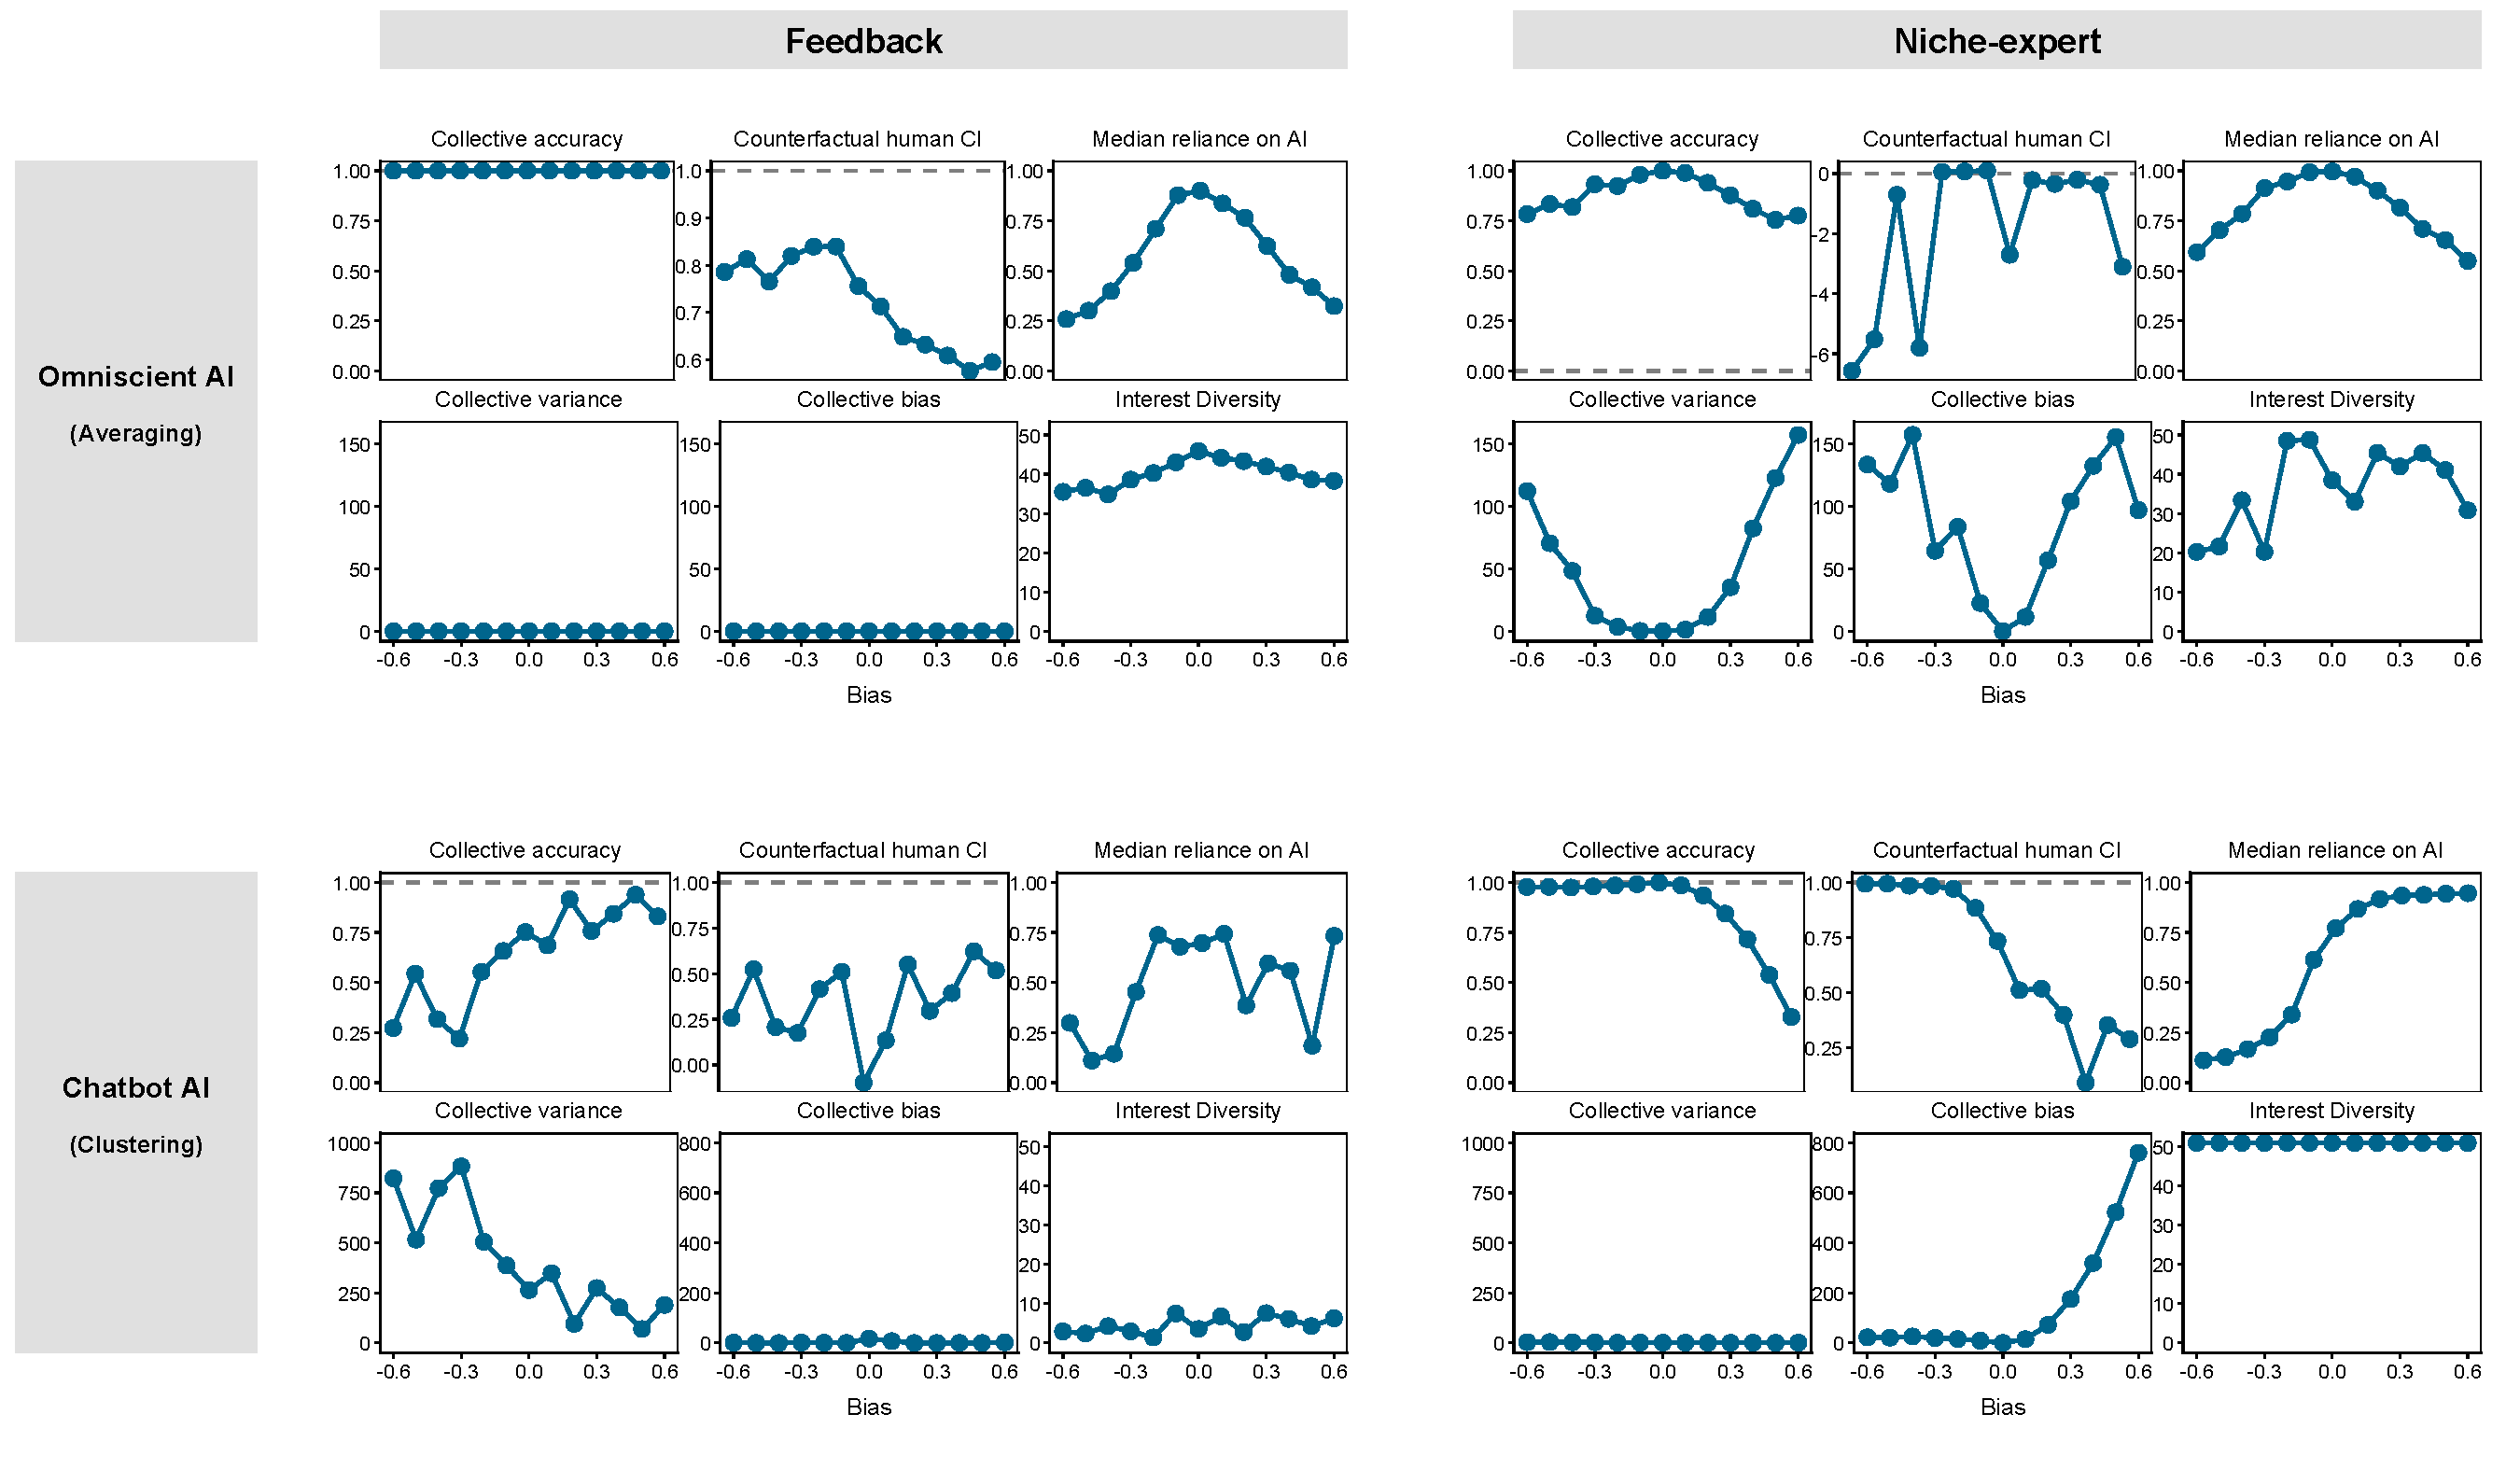
\includegraphics[width=\textwidth]{../Figures/Supplementary figure 1.pdf}
\caption{
\textbf{Niche-expert structure with averaging aggregation cannot promote CI without AI.}
Trajectories of the mean absolute error from true coefficients and collective accuracy under the niche-expert structure with averaging aggregation in the absence of AI.
The mean absolute error from true coefficients is calculated by first taking, for each interest, the absolute difference between the true coefficient and the mean belief of individuals sharing that interest, and then averaging these differences across all $M+1$ interests.
The mean absolute error decreases across generations, indicating that the mean beliefs move closer to their corresponding true coefficients.
However, collective accuracy remains near zero, indicating that simply averaging individual predictions does not yield accurate collective predictions.
Prediction target parameters: $M = 50$, $s = 50$, $\mu = 0$, $\alpha_i \sim U(-5, 5)$, and $\sigma_i \sim U(0, 3)$.
Population parameters: $N = 10{,}000$, $c_A \sim \mathcal{N}(0, 100^2)$.
}
\end{figure}

\pagebreak

\begin{figure}[!pth]
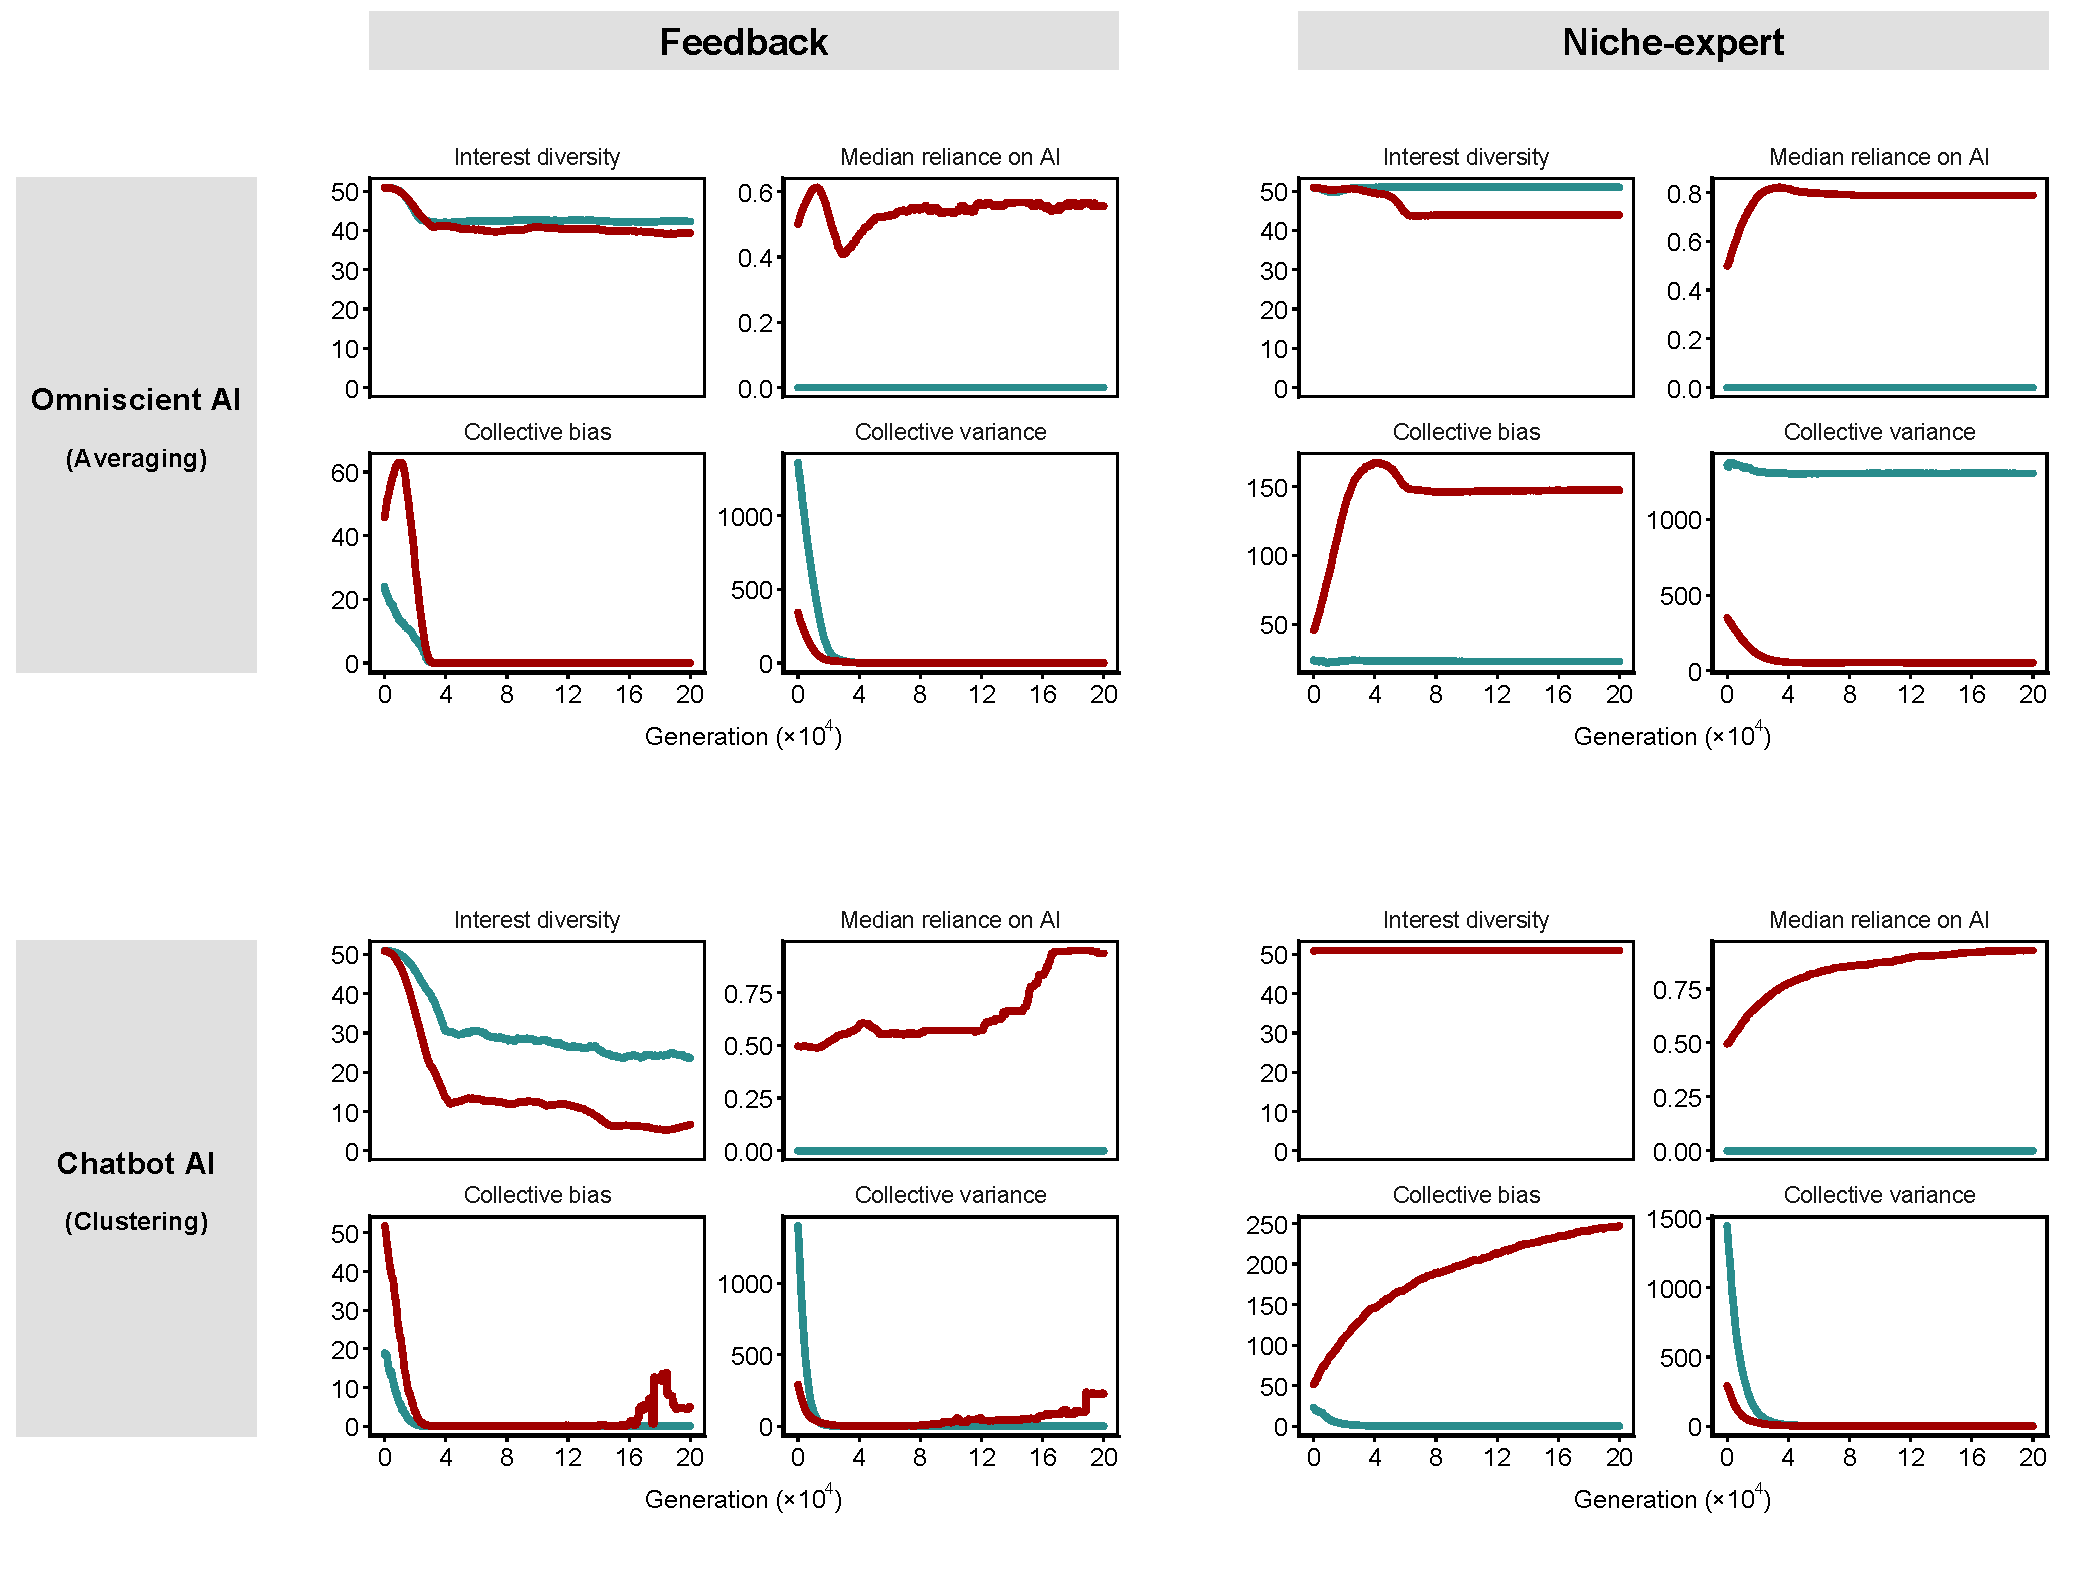
\includegraphics[width=\textwidth]{../Figures/Supplementary figure 2.pdf}
\caption{
\textbf{Evaluation metrics across various levels of AI bias.}
Evaluation metrics across varying levels of AI bias under different assumptions about AI types (Omniscient AI, and Chatbot AI) and incentive structures (feedback, niche-expert).
Larger absolute AI bias indicates a less accurate AI model. 
Dashed horizontal lines represent the values of the evaluation metrics when the group is not assisted by AI.
Collective accuracy represents the predictive performance of the group, and counterfactual human CI represents the group's predictive accuracy if AI assistance were unavailable at the given generation.
Interest diversity is defined as Hill-Shannon diversity of interest within the population, median reliance on AI represents the median value of reliance on AI ($\beta$).
Collective bias represents systematic deviation of the collective prediction from the true target, collective variance represents variability of the collective prediction error across prediction events.
All the evaluation metrics are averaged over generations 190,001--200,000.
Prediction target parameters: $M = 50$, $s = 50$, $\mu = 0$, $\alpha_i \sim U(-5, 5)$, and $\sigma_i \sim U(0, 3)$.
Population parameters: $N = 10{,}000$, $c_A \sim \mathcal{N}(0, 100^2)$ for (A, B), $c_A \sim \mathcal{N}(0, 5^2)$ for (C, D), and $\beta_A \sim U(0, 1)$. 
AI parameters: $\tau = 0.3$.
}
\end{figure}

\pagebreak

\begin{figure}[!pth]
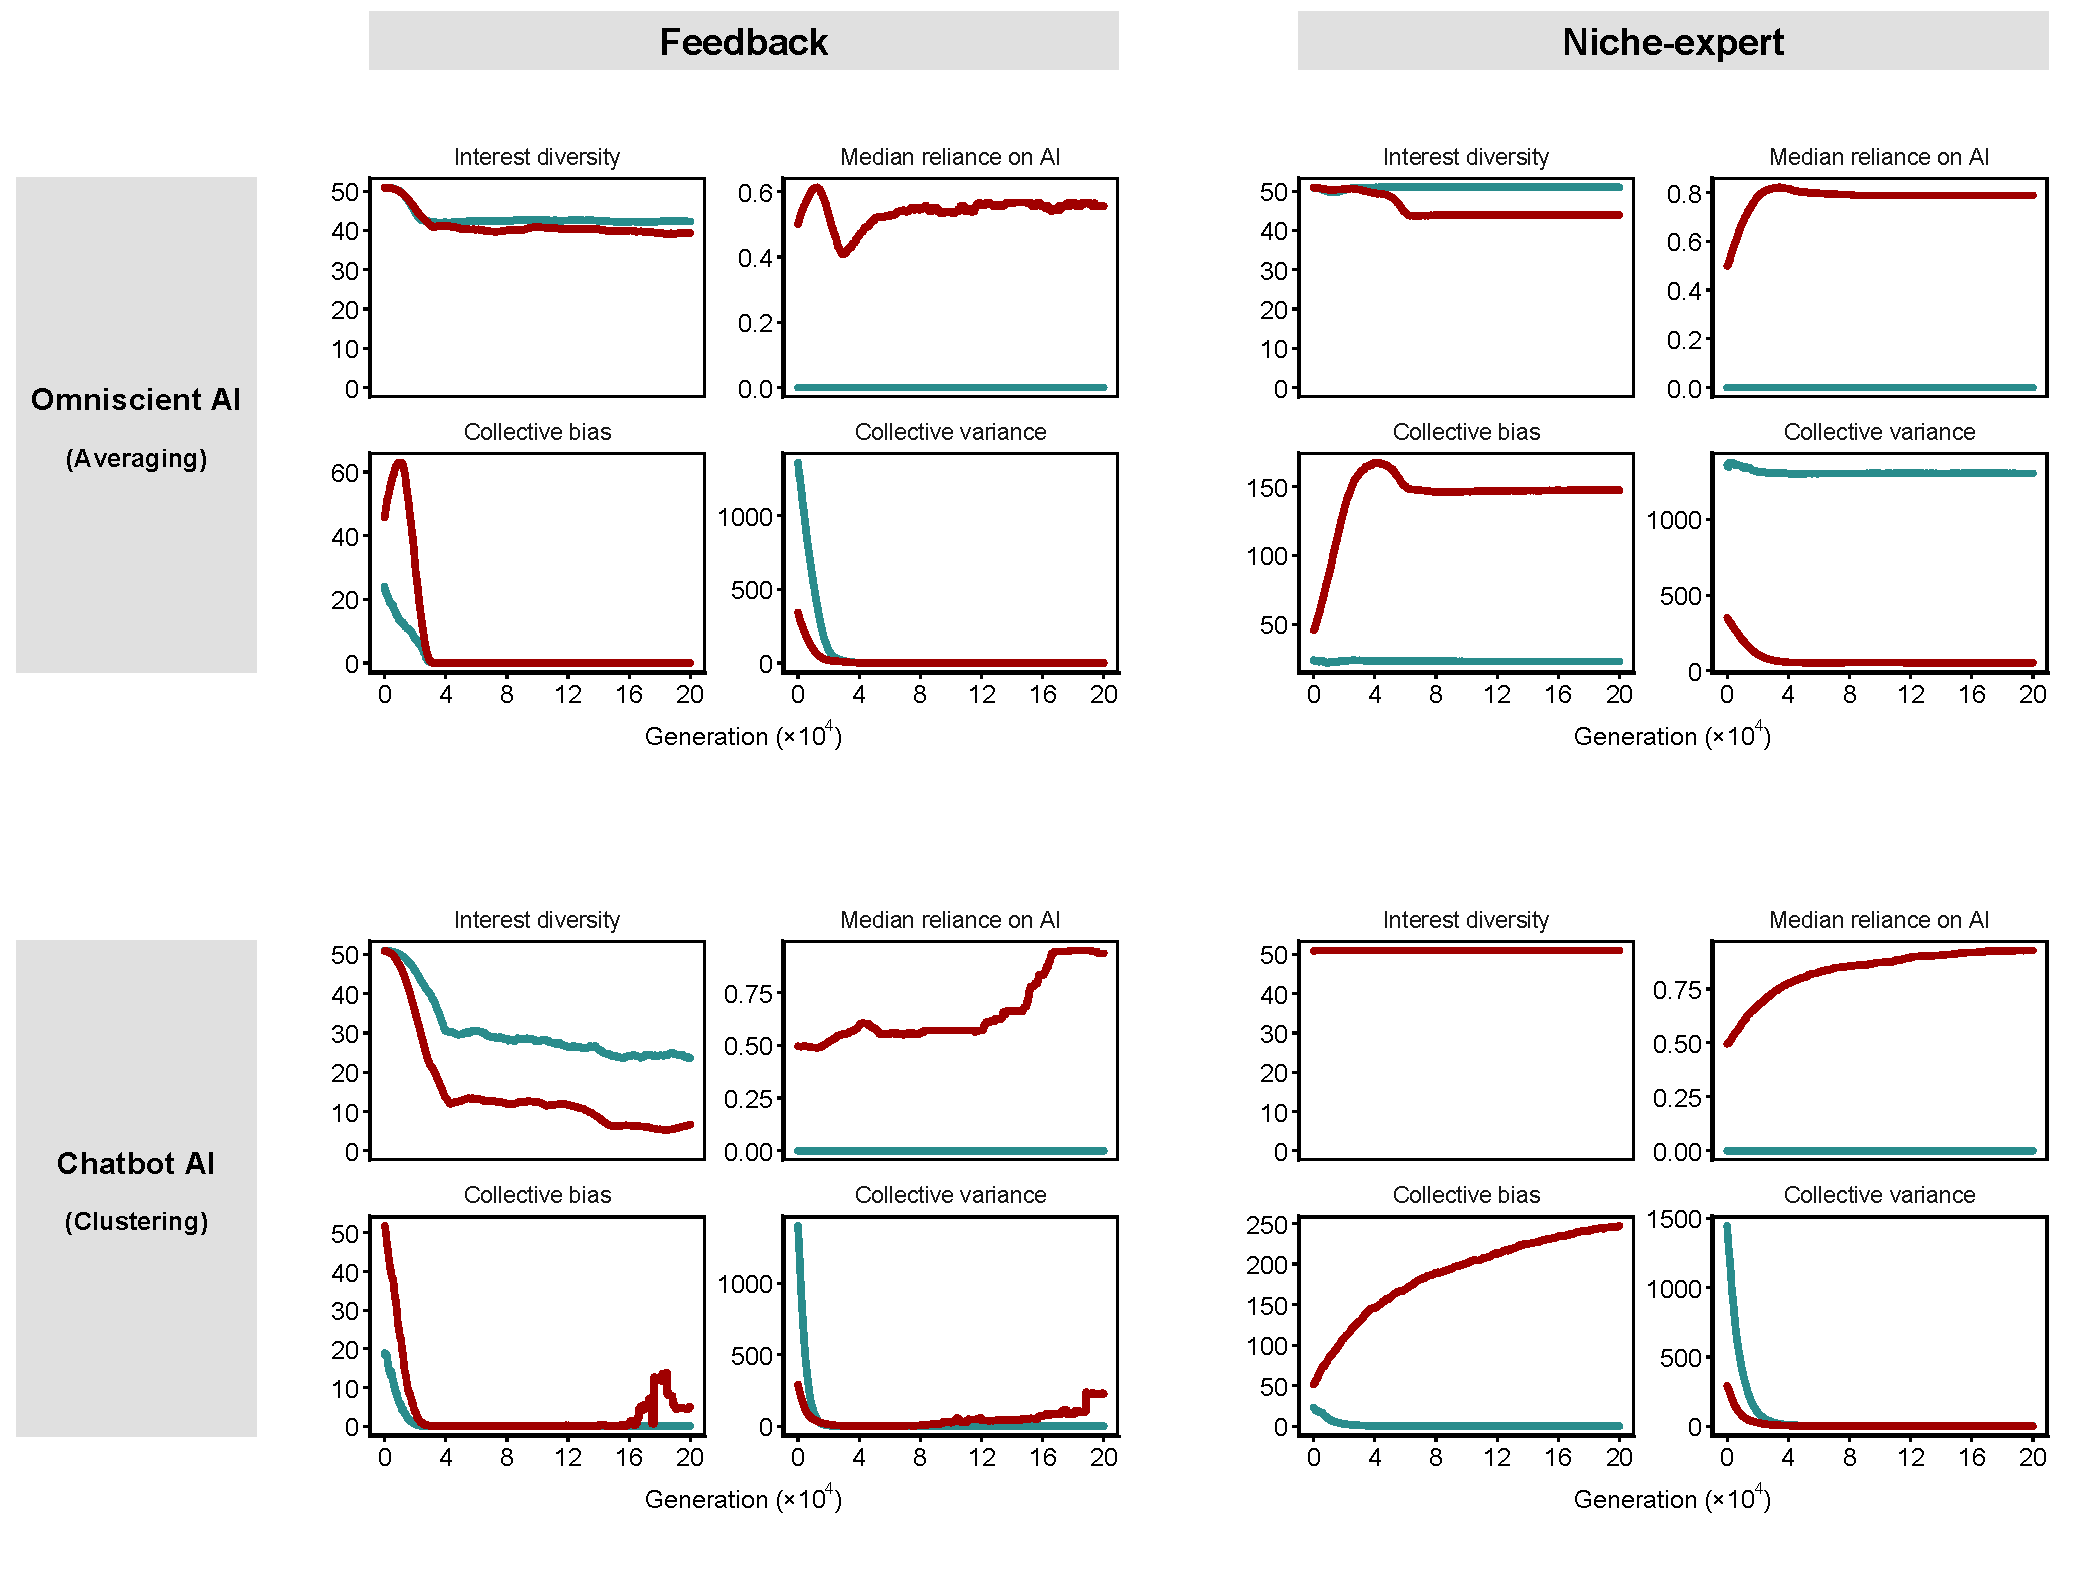
\includegraphics[width=\textwidth]{../Figures/Supplementary figure 3.pdf}
\caption{
\textbf{Comparison of evaluation metrics with and without AI.}
Trajectories of evaluation metrics when the group is assisted by the Omniscient AI and Chatbot AI.
Here, feedback and niche-expert incentive structures are considered.
Blue lines represent trajectories of evaluation metrics without AI assistance.
Orange lines represent trajectories of evaluation metrics with AI assistance.
Interest diversity is define as Hill-Shannon diversity of interest within population, median reliance on AI represent population median of reliance on AI ($\beta$),
collective bias represent systematic deviation of the collective prediction from the true target, collective variance represent variability of the collective prediction error across prediction events.
Prediction target parameters: $M = 50$, $s = 50$, $\mu = 0$, $\alpha_i \sim U(-5, 5)$, and $\sigma_i \sim U(0, 3)$.
Population parameters: $N = 10{,}000$, $c_A \sim \mathcal{N}(0, 100^2)$ for (A, B), $c_A \sim \mathcal{N}(0, 5^2)$ for (C, D), and $\beta_A \sim U(0, 1)$. 
AI parameters: $b_i = 0.4$ and $\tau = 0.3$.
}
\end{figure}

\pagebreak

\begin{figure}[!pth]
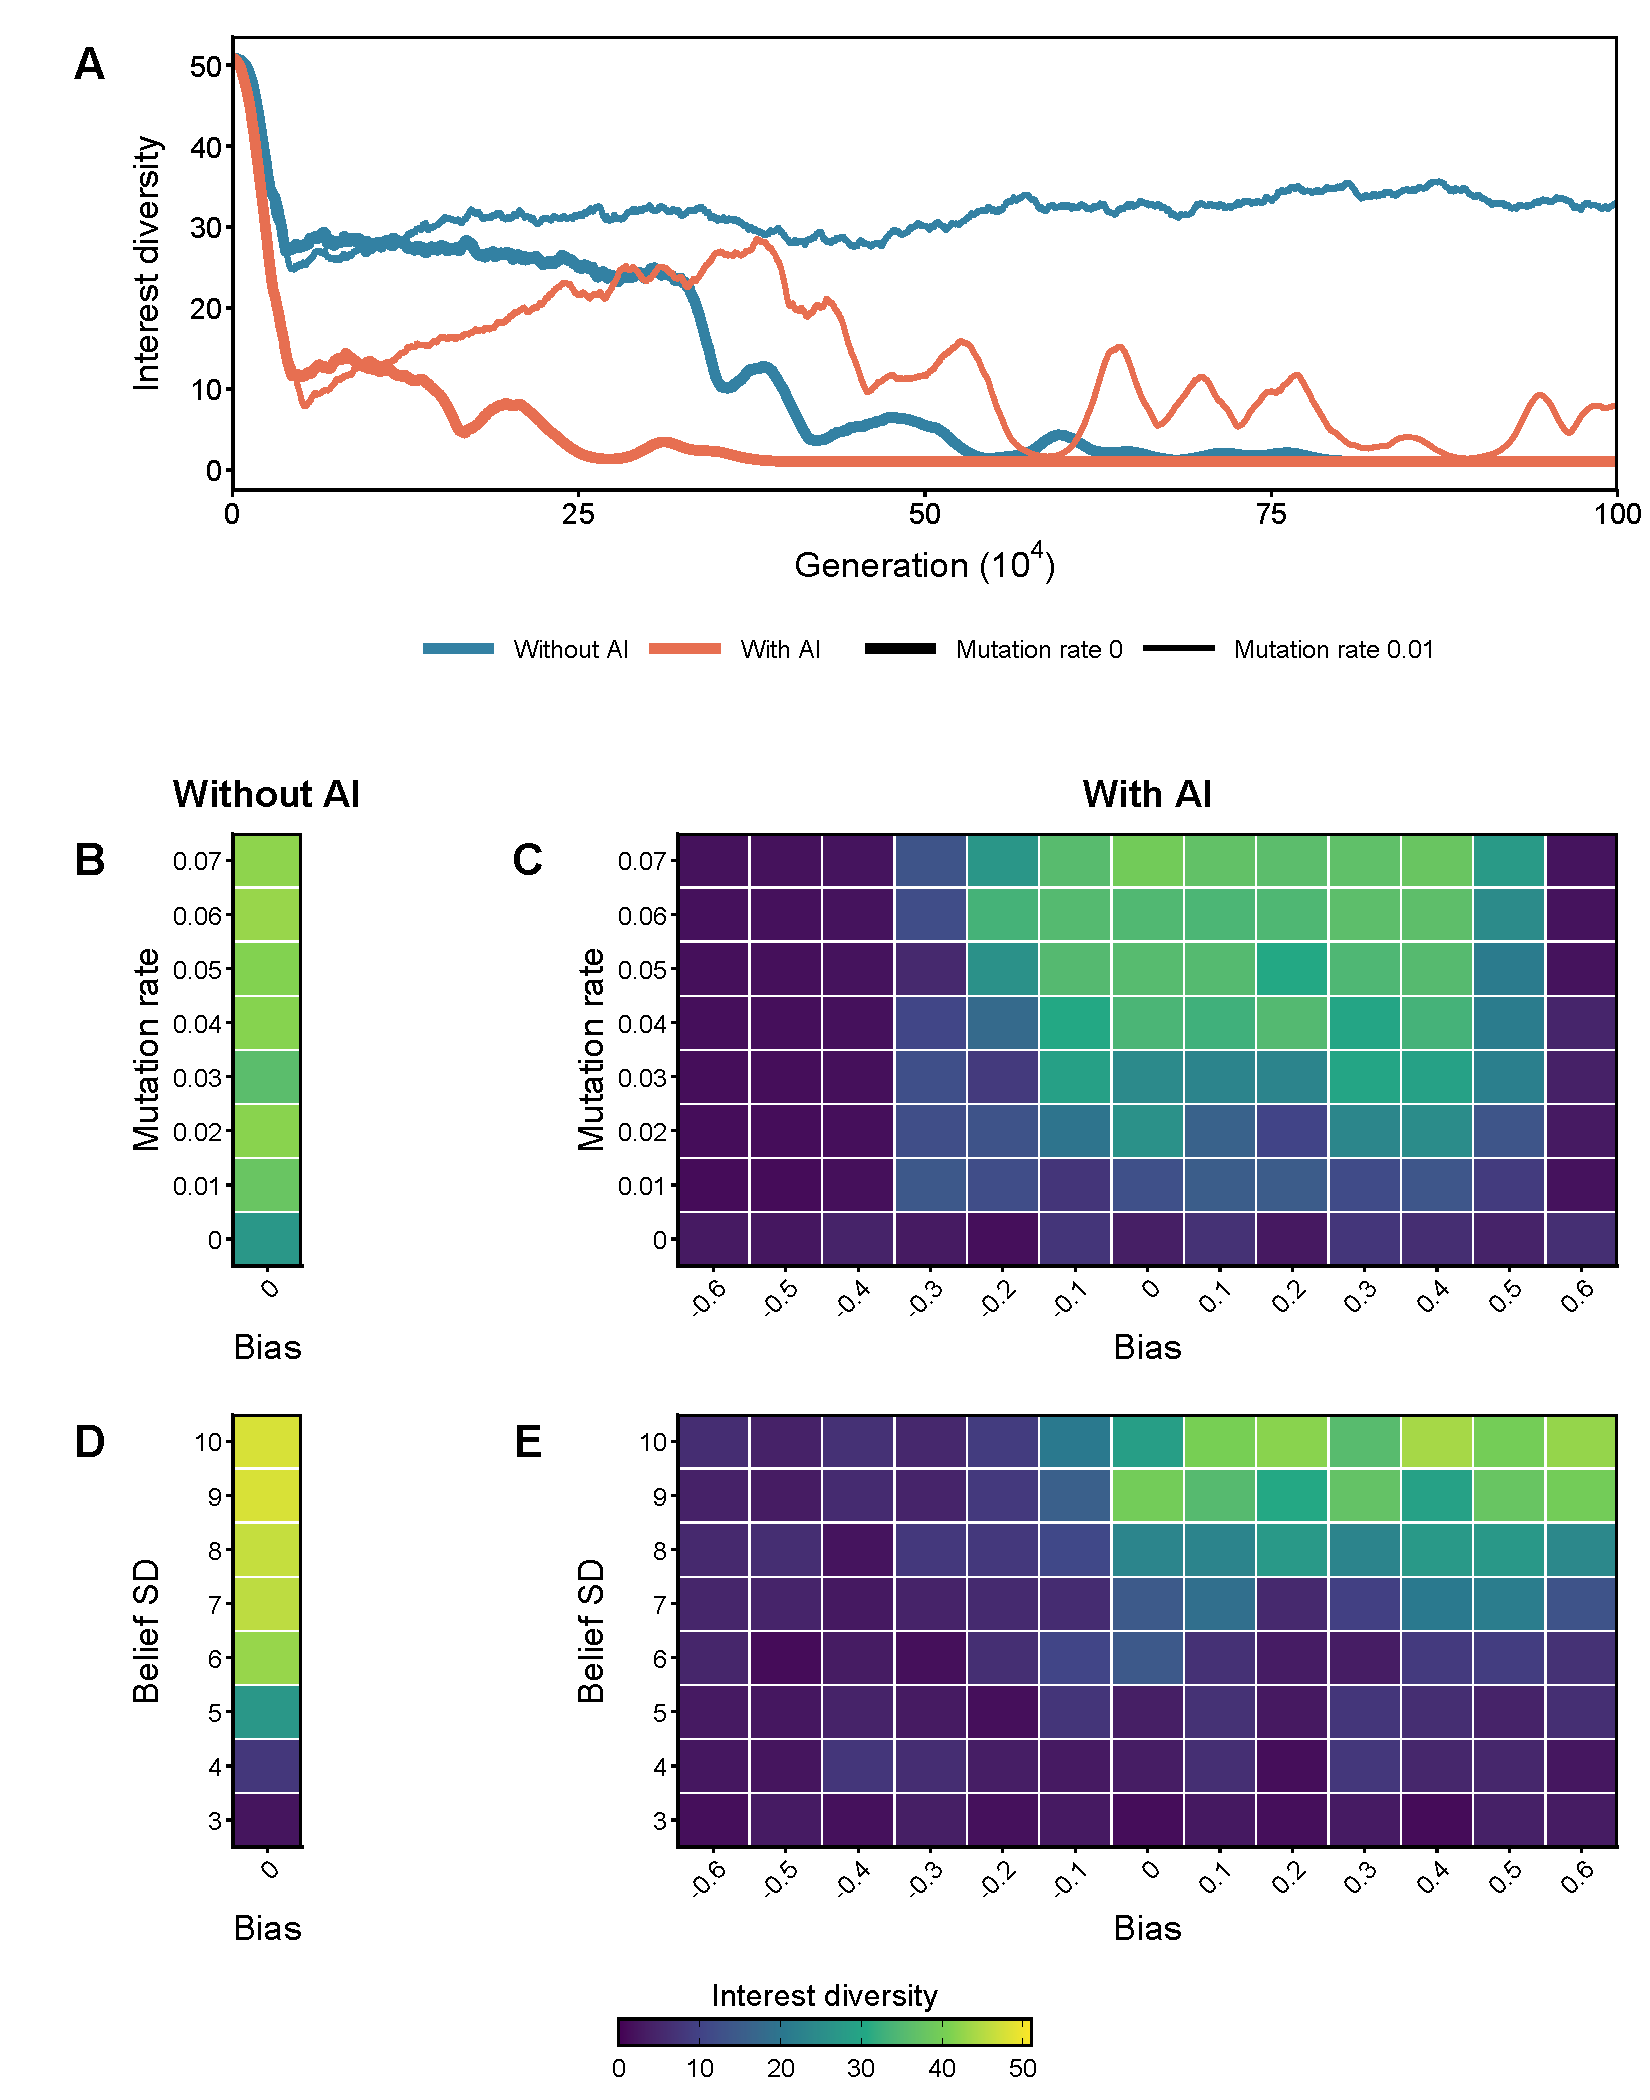
\includegraphics[width=\textwidth]{../Figures/Supplementary figure 4.pdf}
\end{figure}
\pagebreak
\begin{figure}[!pth]
\caption{
\textbf{Feedback structure becomes more prone to interest diversity loss with AI}
Trajectories of interest diversity with and without AI under the feedback structure (A).
Heatmaps of interest diversity across varying levels of mutation rate (B, C) and the standard deviation of the initial belief distribution (D, E), with and without AI.
Interest diversity declines toward zero even without AI over long timescales when there is no mutation and the initial belief distribution is narrow.
However, with AI, interest diversity declines more strongly, even under moderate mutation rates and wider initial belief distributions.
Interest diversity in the heatmaps is averaged over generations 190,001--200,000.
Prediction target parameters: $M = 50$, $s = 50$, $\mu = 0$ for (D, E), $\alpha_i \sim U(-5, 5)$, and $\sigma_i \sim U(0, 3)$.
Population parameters: $N = 10{,}000$, $c_A \sim \mathcal{N}(0, 5^2)$ for (A, B, C), and $\beta_A \sim U(0, 1)$. 
AI parameters: $b_i = 0.4$ and $\tau = 0.3$, Chatbot AI is used.
}
\end{figure}

\pagebreak

\begin{figure}[!pth]
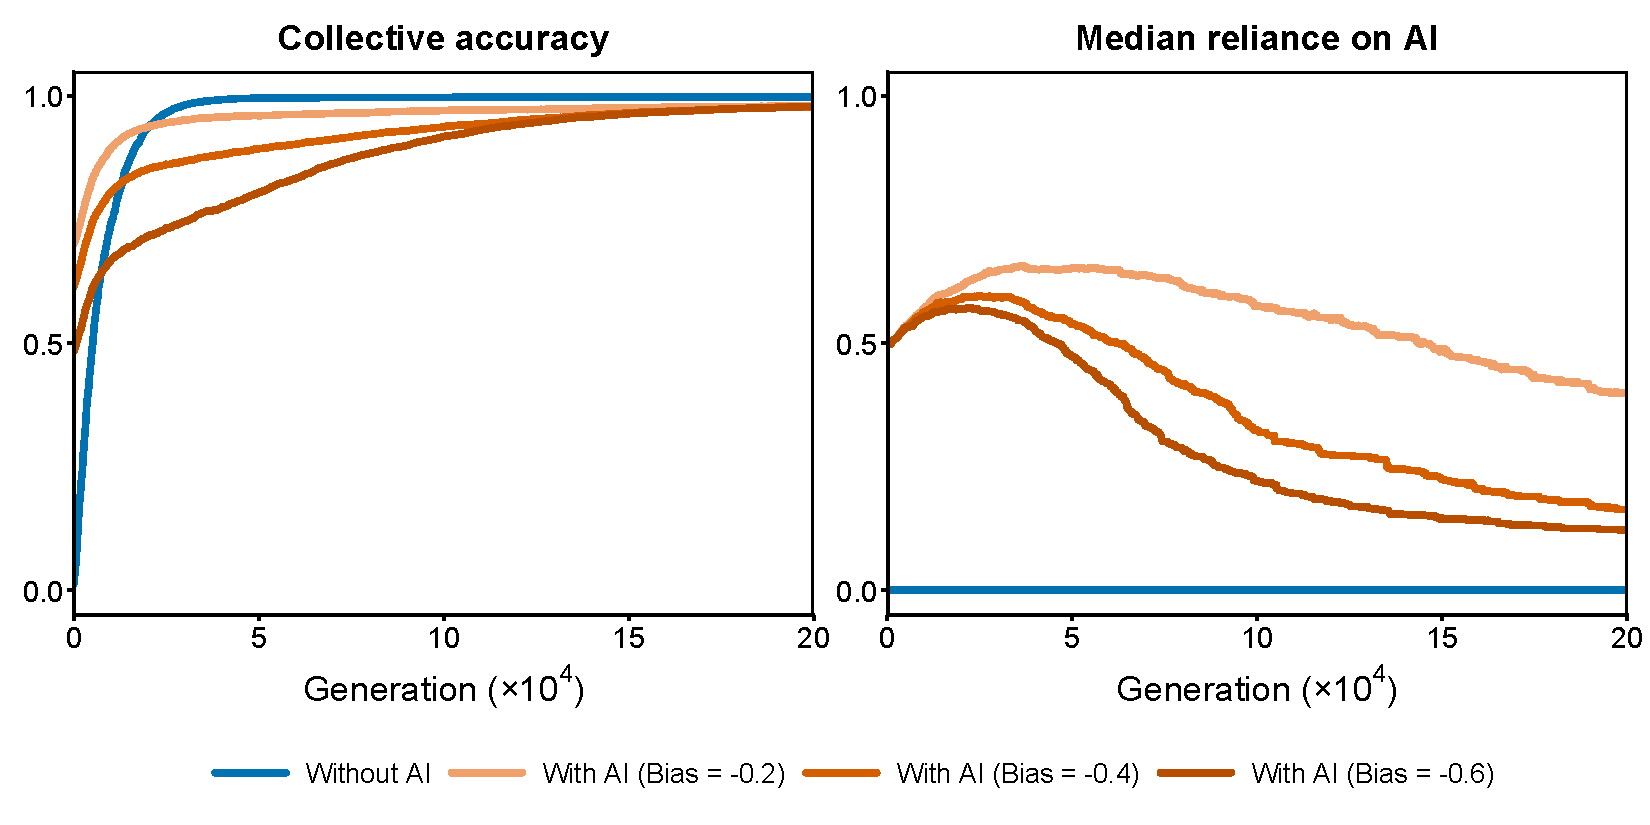
\includegraphics[width=\textwidth]{../Figures/Supplementary figure 5.pdf}
\caption{
\textbf{Niche-expert structure may reduce reliance on AI, delaying the emergence of CI.}
Trajectories of collective accuracy and median reliance on AI when the niche-expert structure causes reliance on AI to decline over time.
Red lines represent trajectories with AI across varying levels of AI bias (-0.2, -0.4, and -0.6).
Green lines represent trajectories without AI; reliance on AI is set to zero in the absence of AI.
This reduction in reliance on AI occurs when the $\alpha_0$ and AI bias have opposite signs, and is associated with the eventual emergence of CI, although CI emerges substantially later than in the condition without AI.
Prediction target parameters: $M = 50$, $s = 50$, $\mu = 0$, $\alpha_i \sim U(-5, 5)$, and $\sigma_i \sim U(0, 3)$.
Population parameters: $N = 10{,}000$, $c_A \sim \mathcal{N}(0, 5^2)$, and $\beta_A \sim U(0, 1)$. 
AI parameters: $\tau = 0.3$, Chatbot AI is used.
}
\end{figure}


\pagebreak

\begin{figure}[!pth]
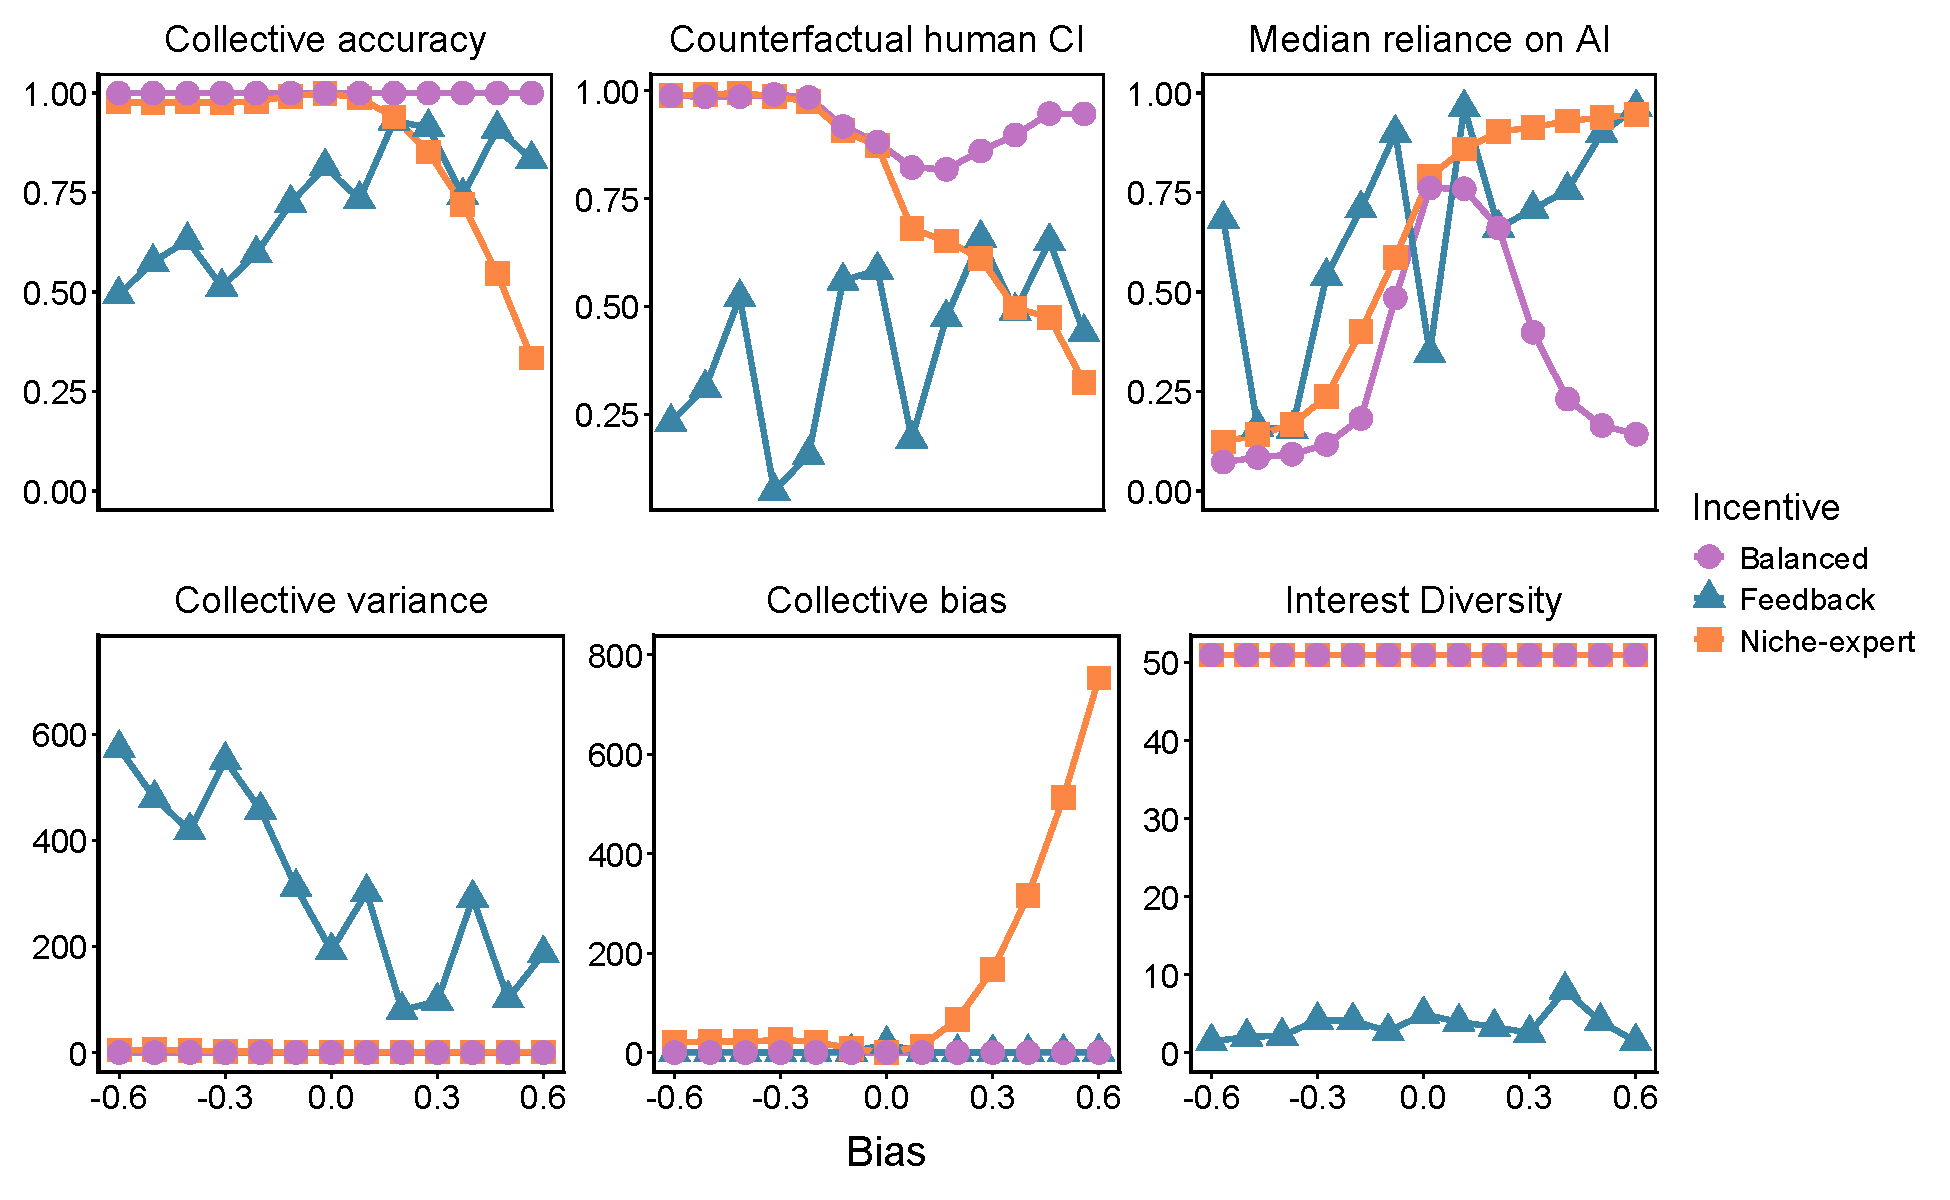
\includegraphics[width=\textwidth]{../Figures/Supplementary figure 6.pdf}
\caption{
\textbf{Comparison of evaluation metrics between incentive structures across various levels of AI bias.}
Evaluation metrics under feedback, niche-expert and balanced structures across varying levels of AI bias.
Larger absolute AI bias indicates a less accurate AI model. 
All the evaluation metrics are averaged over generations 190,001--200,000.
The balanced structure maintains near-perfect collective accuracy across bias levels and higher counterfactual human CI than the other incentive structures.
These patterns are driven by well-calibrated reliance on AI, which increases as AI becomes more accurate, and by well-preserved interest diversity, which together lead to low collective variance and collective bias.
Prediction target parameters: $M = 50$, $s = 50$, $\mu = 0$, $\alpha_i \sim U(-5, 5)$, and $\sigma_i \sim U(0, 3)$.
Population parameters: $N = 10{,}000$, $c_A \sim \mathcal{N}(0, 5^2)$, and $\beta_A \sim U(0, 1)$. 
AI parameters: $\tau = 0.3$, Chatbot AI is used.
}
\end{figure}

\pagebreak

\begin{figure}[!pth]
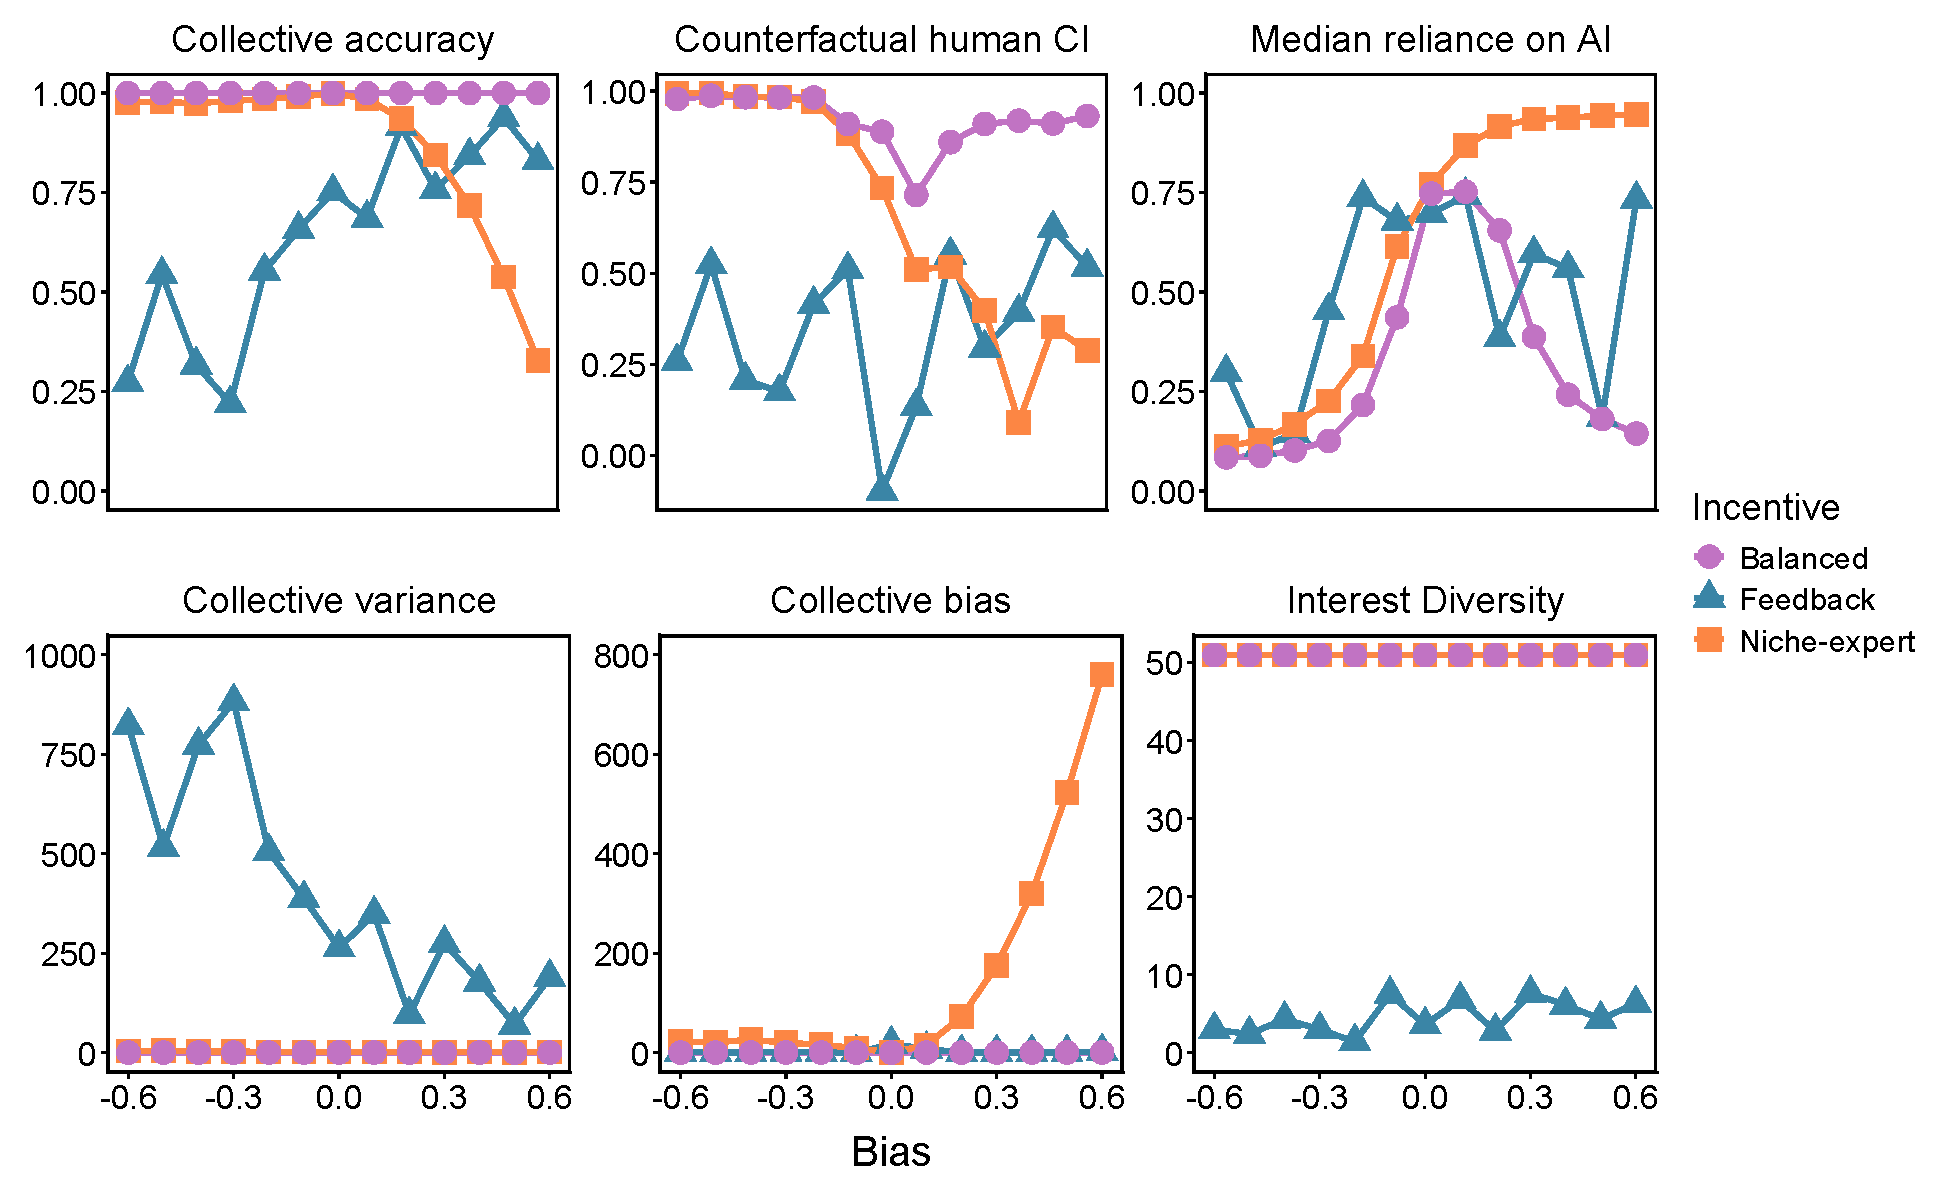
\includegraphics[width=\textwidth]{../Figures/Supplementary figure 7.pdf}
\caption{
\textbf{Balanced structure is robust across varying balancing weights.}
Evaluation metrics across varying levels of the balancing weight (0.1 -- 0.9).
The balancing weight represents the weight assigned to the niche-expert structure when constructing the balanced structure by combining the niche-expert and feedback structures.
A balancing weight of 0.5 represents equal weighting of the niche-expert and feedback structures, whereas 0 corresponds to the feedback structure and 1 corresponds to the niche-expert structure.
Although the evaluation metrics vary as the balancing weight changes from 0.1 to 0.9, the absolute magnitude of these deviations remains limited.
Prediction target parameters: $M = 50$, $s = 50$, $\mu = 0$, $\alpha_i \sim U(-5, 5)$, and $\sigma_i \sim U(0, 3)$.
Population parameters: $N = 10{,}000$, $c_A \sim \mathcal{N}(0, 5^2)$, and $\beta_A \sim U(0, 1)$. 
AI parameters: $b_i = 0.4$, $\tau = 0.3$, Chatbot AI is used.
}
\end{figure}

\pagebreak

\begin{figure}[!pth]
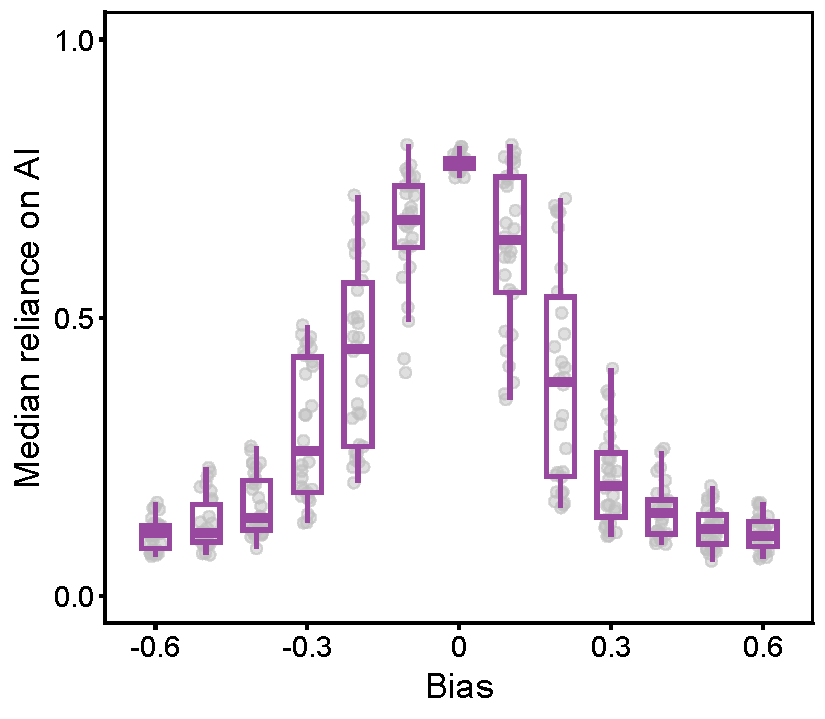
\includegraphics[width=\textwidth]{../Figures/Supplementary figure 8.pdf}
\caption{
\textbf{Balanced structure shows well-calibrated reliance on AI.}
Median reliance on AI across varying levels of AI bias.
Thirty randomly initialized simulations were performed for each bias level.
Each dot represents a single simulation, and the box plots show the median and interquartile range (IQR) for each bias level.
The balanced structure shows well-calibrated reliance on AI, with reliance increasing as absolute magnitude of AI bias decreases.
Prediction target parameters: $M = 50$, $s = 50$, $\mu = 0$, $\alpha_i \sim U(-5, 5)$, and $\sigma_i \sim U(0, 3)$.
Population parameters: $N = 10{,}000$, $c_A \sim \mathcal{N}(0, 5^2)$, and $\beta_A \sim U(0, 1)$. 
AI parameters: $\tau = 0.3$, Chatbot AI is used.
}
\end{figure}

\pagebreak

\begin{figure}[!pth]
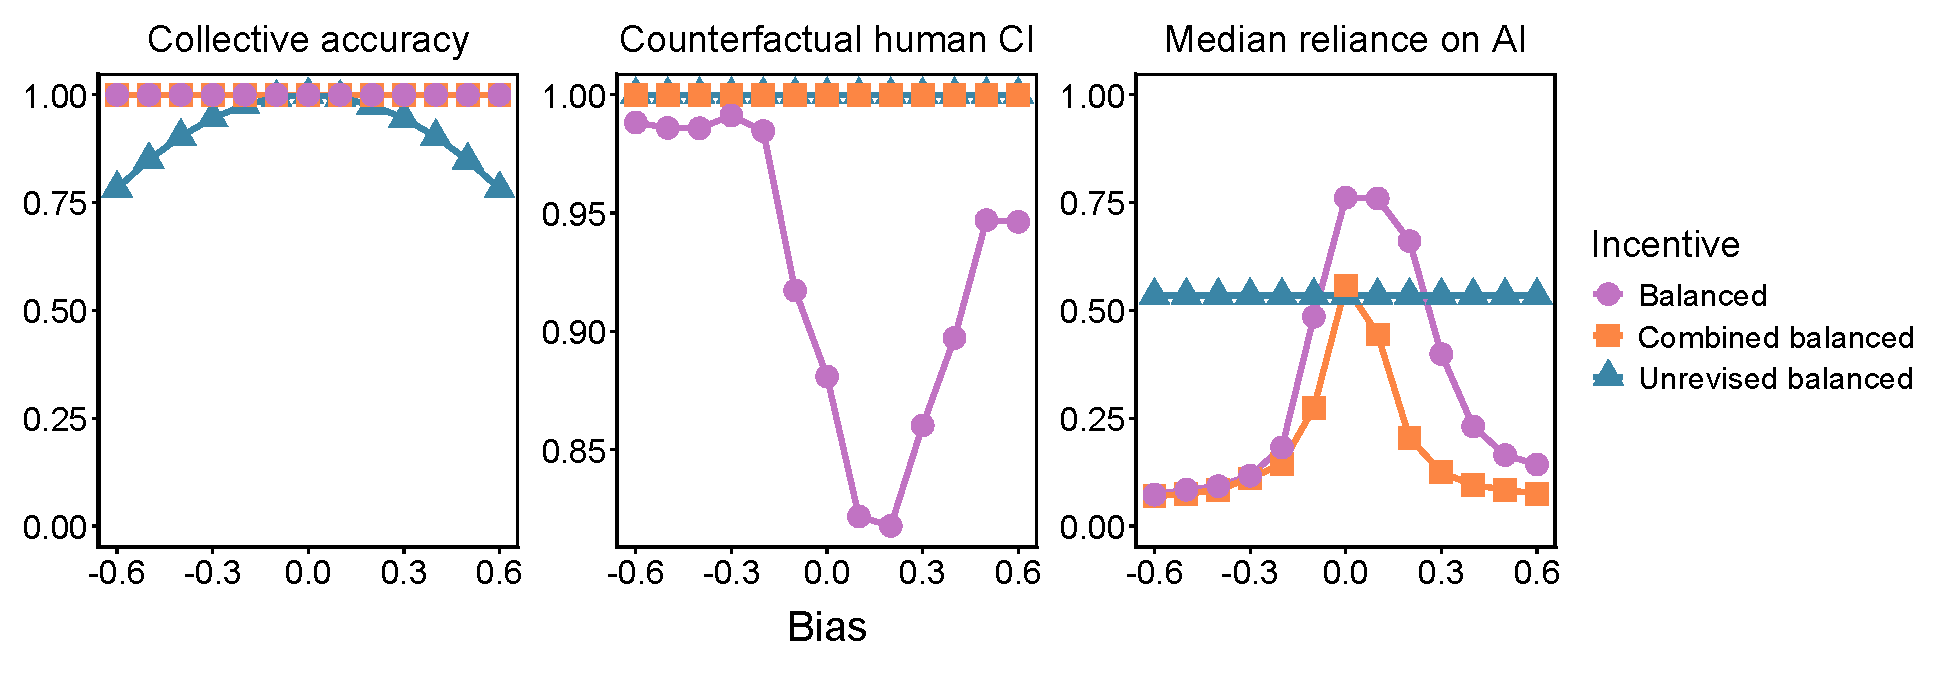
\includegraphics[width=\textwidth]{../Figures/Supplementary figure 9.pdf}
\caption{
\textbf{Incentive structures incorporating unrevised prediction accuracy can promote better counterfactual human CI.}
Evaluation metrics under the balanced, unrevised balanced, and combined balanced structures across varying levels of AI bias.
The unrevised balanced structure is defined as the arithmetic mean of the feedback and niche-expert structures based on unrevised predictions, whereas the combined balanced structure is defined as the arithmetic mean of the balanced and unrevised balanced structures.
All evaluation metrics are averaged over generations 190,001--200,000.
The unrevised balanced structure achieves near-perfect counterfactual human CI; however, median reliance on AI remains near 0.5 because the unrevised balanced incentive does not account for AI predictions and therefore imposes no selection on $\beta_A$.
Consequently, collective accuracy directly inherits AI bias and decreases as the magnitude of AI bias increases.
The combined balanced structure, which leverages both the balanced and unrevised balanced structures, achieves near-perfect counterfactual human CI without compromising collective accuracy.
Prediction target parameters: $M = 50$, $s = 50$, $\mu = 0$, $\alpha_i \sim U(-5, 5)$, and $\sigma_i \sim U(0, 3)$.
Population parameters: $N = 10{,}000$, $c_A \sim \mathcal{N}(0, 5^2)$, and $\beta_A \sim U(0, 1)$.
AI parameters: $\tau = 0.3$; Chatbot AI is used.
}
\end{figure}

\pagebreak

\begin{figure}[!pth]
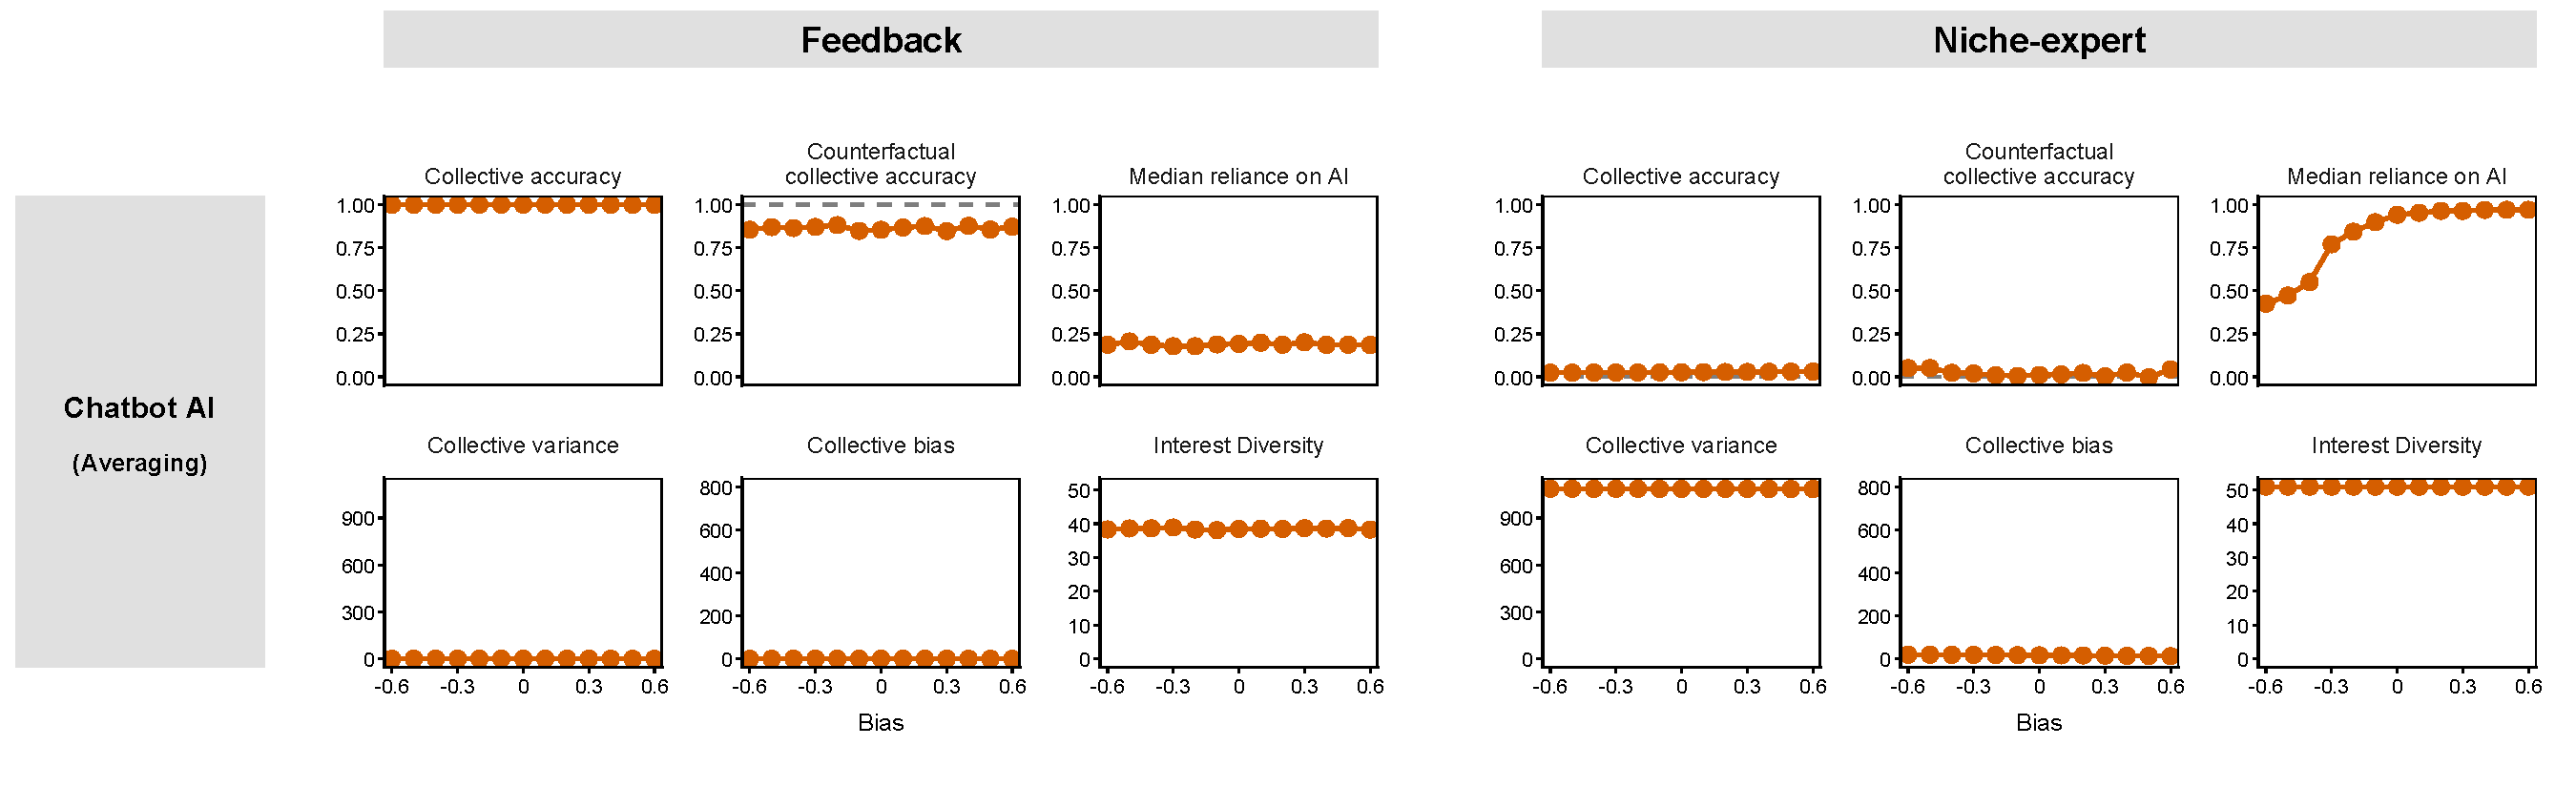
\includegraphics[width=\textwidth]{../Figures/Supplementary figure 10.pdf}
\caption{
\textbf{Chatbot AI with averaging aggregation has a limited influence on CI.}
Evaluation metrics across varying levels of AI bias under Chatbot AI with averaging aggregation.
Two incentive structures, feedback and niche-expert, are considered.
A larger absolute AI bias indicates a less accurate AI model.
Dashed horizontal lines represent the values of the evaluation metrics when the group is not assisted by AI.
Collective accuracy represents the predictive performance of the group, whereas counterfactual human CI represents the group's predictive accuracy if AI assistance were unavailable at the given generation.
Interest diversity is defined as the Hill--Shannon diversity of interests within the population, and median reliance on AI represents the median reliance on AI ($\beta$) across individuals.
Collective bias represents the systematic deviation of the collective prediction from the true target, whereas collective variance represents the variability of collective prediction errors across prediction events.
All evaluation metrics are averaged over generations 190,001--200,000.
Prediction target parameters: $M = 50$, $s = 50$, $\mu = 0$, $\alpha_i \sim U(-5, 5)$, and $\sigma_i \sim U(0, 3)$.
Population parameters: $N = 10{,}000$, $c_A \sim \mathcal{N}(0, 100^2)$, and $\beta_A \sim U(0, 1)$.
AI parameters: $\tau = 0.3$.
}
\end{figure}

\pagebreak


\begin{table}[htbp]
\centering
\caption{Evaluation metrics used to analyze collective prediction dynamics.}
\label{tab:evaluation_metrics}
\renewcommand{\arraystretch}{1.25}
\begin{tabularx}{\textwidth}{@{}L{0.28\textwidth} C{0.27\textwidth} Y@{}}
\toprule
Metric & Definition & Interpretation \\
\midrule

Collective accuracy &
\(\displaystyle 1-\frac{\mathbb{E}[(Y-\hat{Y}^{\mathrm{re}})^2]}{\mathbb{E}[(Y-\alpha_0)^2]}\) &
Accuracy of the revised collective prediction relative to the baseline prediction $\alpha_0$. \\
\addlinespace

Collective bias &
\(\displaystyle \left(\mathbb{E}[Y-\hat{Y}^{\mathrm{re}}]\right)^2\) &
Squared expected deviation of the revised collective prediction from the true target. \\
\addlinespace

Collective variance &
\(\displaystyle \operatorname{Var}(Y-\hat{Y}^{\mathrm{re}})\) &
Variability of the revised collective prediction error across prediction events. \\
\addlinespace

Counterfactual collective accuracy &
\(\displaystyle 1-\frac{\mathbb{E}[(Y-\hat{Y})^2]}{\mathbb{E}[(Y-\alpha_0)^2]}\) &
Accuracy obtained after removing AI use from the current population while retaining its evolved interests and beliefs. \\
\addlinespace

Interest diversity &
\(\displaystyle \exp\left(-\sum_{i=0}^{M}\rho_i\ln\rho_i\right)\) &
Effective number of interests represented in the population. \\
\addlinespace

Median reliance on AI &
\(\displaystyle \operatorname{median}_{A\in N}(\beta_A)\) &
Median reliance on AI in the population. \\

\bottomrule
\end{tabularx}
\end{table}

\pagebreak

\bibliography{references}


\end{document}
